\setcounter{secnumdepth}{4}
\section{Neural Networks}  \label{cha:foundations_basics_nn}
This section is organized as follows. In this section first providing a brief history of deep learning ...\todo{here you explain why you have only example of an architecture for cnns}
\subsection{The Beginnings of Artificial Neural Networks}
\todo{you can also add activation functions}
%if you like to extend you can add country and the field of the people
Alan Turing who is considered to be the father of computer science and artificial intelligence laid the first foundations of artificial intelligence with his paper titled \textit{"Computing machinery and intelligence"} in 1950s. In his paper he introduced the \textit{Turing test} which is a test of a computer's ability to determine whether it can be regarded as intelligent. During this test a human evaluator, i.e., \textit{referee} judges the computer's ability. 
In the Turing test a referee would have natural language conversations with a person and a computer which is designed to respond human-like. If the referee cannot distinguish between the computer and the person then the machine would pass the test and it might be considered as intelligent. Although this idea was proposed decades ago, today Turing test is still used widely as a benchmark in artificial intelligence. 

The second founding event of artificial intelligence was a \textit{Dartmouth Summer Research Project on Artificial Intelligence}, 1956 Workshop. The Workshop lasted six to eight weeks as brainstorming sessions where McCarthy coined the term "artificial intelligence" in 1955. Several important people in the field of artificial intelligence (e.g., John McCarthy, Marvin Minsky, Julian Bigelow, Donald MacKay, and more besides) participated in the workshop.

On the other hand, Walter Pitts and Warren McCulloch started the history of neural networks with their paper titled \textit{A Logical Calculus of Ideas Immanent in Nervous Activity}\footnote{\url{http://www.cs.cmu.edu/~epxing/Class/10715/reading/McCulloch.and.Pitts.pdf}}.  The paper describes the idea of the artificial neural networks with relevant definitions which we still rely on them today. They split the neurons of a network into two groups, the first group is called \textit{peripheral afferents}, i.e., input neurons and the second group is the output neurons. Back then the concept of \textit{hidden layer} was not introduced. 

Another hero of deep learning is Frank Rosenblatt, an American psychologist. Rosenblatt discovered the famous \textit{perceptron learning rule} which is still today one of the most widely used learning algorithm. The rule explains how to update the parameters (weights) of a neural network while training it. Besides his discovery of perceptron,  Rosenblatt also explored several neural network architectures in his book \textit{Principles of Neurodynamics}~\cite{} and
put forward an idea of multilayered networks that are similar to convolutions neural networks today. This is considered the start of the journey towards \textit{deep learning}. 

Despite of the developments in artificial neural networks,  the book written by Marvin Minsky and Seymour Papert in 1969 caused huge setback. In the book, Minsky and Papert tried to prove that perceptrons are simple linear classifiers and has major computational limitations such as XOR function. Further, the book had great impact on the discouragement of further development of artificial neural networks. Thereafter,  a positive development occurred. The discovery of Backpropagation by Rumelhart, Hinton and Williams enabled the community to train a neural network with more than one layer. However, this discovery neglected by the community. 

In early 1990s, support vector machines (SVMs) gained significant attention due to their performance and simplicity. In fact people from AI community shifted towards them. In the late 1990s, two important improvements occurred which laid the foundations of today's deep neural networks (1) the invention of the long short-term memory by Hochreiter and Schmidhuber in 1997; (2) the design of a first convolutional neural network in 1998 by LeCun, Bottou, Bengio and Haffner and it is called LeNet-5 . Thereafter, in 2006 Hinton, Osindero and Teh published a paper which introduces deep belief networks (DMB). After this paper a new period of AI began.
\subsection{The Basic Architecture of Neural Networks} 
%book:Neural Networks and Deep Learning, Charu C. Aggarwal
In this section, the basic architectures of single-layer and multi-layer neural networks have been discussed. Single-layer neural networks are also referred to as \textit{perceptrons} which have an output layer and the set of inputs are directly mapped to the output layer%you can say only a node. 
. Moreover, multi-layer neural networks which do not have only input and output layers but also hidden layers. This type of neural networks is also known as \textit{feed-forward networks}. 
%This chapter aims for providing an overview on the
\subsubsection{Single-layer Neural Networks: Perceptrons}
\begin{figure}[t]
%\centering

%\captionsetup{justification=centering, margin={0cm,0.5cm}}
\begin{subfigure}[t]{.5\textwidth}
  \centering
  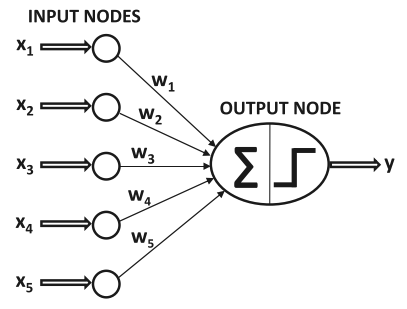
\includegraphics[width=\linewidth]{Figures/fig_perceptron_wo_bias.png}
  \caption{Perceptron without bias}
  \label{fig:perceptron_wo_bias}
\end{subfigure}%
\hspace{0.5cm}
\begin{subfigure}[t]{.5\textwidth}
  %\centering
  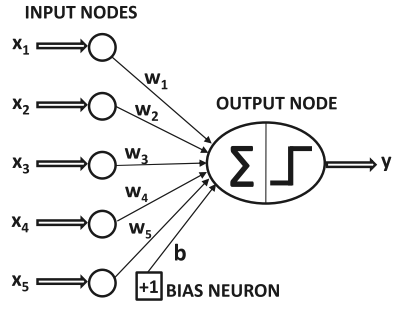
\includegraphics[width=\linewidth]{Figures/fig_perceptron_w_bias.png}
  \caption{Perceptron with bias}
  \label{fig:perceptron_w_bias}
\end{subfigure}
 \caption{An overview of perceptron architectures. The image is extracted from~\protect\cite{DBLP:books/sp/Aggarwal18}} 
  \label{fig:whole_perceptron}
  %\cref{fig:whole_karate_network_representation}
\end{figure}
% \begin{figure*}[t]
% \centering
%  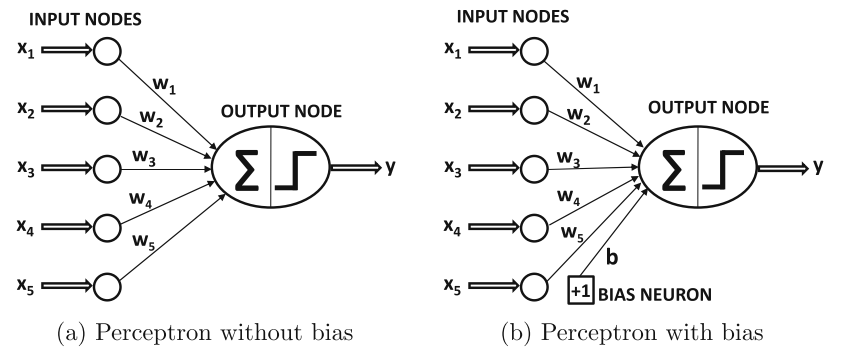
\includegraphics[width=\linewidth]{Figures/fig_perceptron.png}
%  \caption{An overview of perceptron architectures. The image is extracted from~\protect\cite{DBLP:books/sp/Aggarwal18}.}
%  \label{fig:perceptron}
% \end{figure*} \\
Perceptrons have the plainest architecture of neural networks. It consists of only an input and output layer. The output layer contains only a single node which produces the final output value. Figure~\ref{fig:whole_perceptron} illustrates \todo{fix figure caption} perceptron architectures with and without a bias neuron. The bias value improves the performance of the network, in other words, enables network to make more accurate predictions. Moreover, in order to incorporated bias into neural network, an additional input neuron called \textit{bias neuron} which transmits the value 1 to the next layer is added. 

The given input features are $x_1, x_2, ..., x_5$ (cf. Figure~\ref{fig:whole_perceptron}) and the input layer simply transmits the each individual feature to the output layer by multiplying them with their corresponding weight. For example, $x_1$ is multiplied with $w_1$, $x_2$ is multiplied with $w_2$ and so on. In a general neural network architecture the input layer does not perform any computation, and thus often, it is not included in the count of the number of layers.

Given a training set where each instance is of a form ($\overline{X}$, $y$), where $\overline{X}=[x_1,x_2,...,x_d]$ denotes an input variable with \textit{d}-dimensional features and $y$ is the actual label of  $\overline{X}$ such that $y \in{\{-1, +1\}}$. Let $\overline{W}=[w_1,w_2,...,w_d]$ denote the weight of the edges and $b$ is a bias. Then, the output $\hat{y}$ is computed as follows: \begin{equation} \label{eq:perceptro}
\hat{y}=sign\{ \overline{W}\cdot \overline{X}+b\} = sign\{ \sum\limits_{j=1}^{d} w_jx_j+b\}
\end{equation}


The sign function maps a real value to either \num{+1} or \num{-1} as $y \in{\{-1, +1\}}$. In other words, the sign function here serves the role of an \textit{activation function}. Generally, the activation function can be defined as follows: Given a set of inputs to a node the activation function defines the output of that node. Depending on the application at hand different type of activation functions such as \textit{sigmoid, ReLU, softmax} can be utilized. The formalized (cf. Equation~\ref{eq:perceptro}) scenario is appropriate for binary classification task where the output of the sign function, i.e., \num{-1} or \num{+1} corresponds to a class label (e.g., spam or not spam). 

By the time Rosenblatt proposed perceptron algorithm, the optimization process of a network is performed heuristically. Therefore, there were not any formal definition of a loss function for perceptrons like we have today for any machine learning algorithm. However, the goal of the heuristic function was the same as today's loss functions, minimizing the number of miss classified samples, i.e., minimizing the error in predictions. However, today several resources related to perceptrons formalize this heuristic learning process. Following we give the heuristically motivated loss function in least-squares form with respect to all training instances:
\begin{equation}
    Minimize_{\overline{W}} L=\sum\limits_{(\overline{X},y) \in D}(y-\hat{y})^2 = \sum\limits_{(\overline{X},y) \in D}(y-sign\{\overline{W}\cdot\overline{X}\})^2 .
    \label{eq:loss_perceptron}
\end{equation}
The key idea here is finding the optimal weight values $\overline{W}$ which minimizes the Equation~\ref{eq:loss_perceptron}. 

% The weights then updated based on the error value as follows:
% %Formula 1.3
% \begin{equation}
%     \nabla L=\sum\limits_{(\overline{X},y) \in D}(y-\hat{y})\overline{X}
%     \label{eq:perceptron_weight_error_value}
% \end{equation}
% where $D$ denotes the entire training data. Note that the above function is defined over the entire training data. 

Typically, this type of a neural network is trained by feeding each input data instance $\overline{X}$ one by one to create the prediction $\hat{y}$. Then the weights are updated in each iteration based on the error value $E(\overline{X}) = (y-\hat{y})$ as follows:
%Formula 1.4
\begin{equation}
    \overline{W} \Leftarrow \overline{W} \alpha (y-\hat{y})\overline{X}
\end{equation}
where $\alpha$ denotes the learning rate of the neural network. Finally, the weights are updated iteratively until the convergence is reached. 

The introduced perceptron model is a type of a linear classifier which defines a linear hyperplane between the data points. Ideally, the data points belong to the same class falls on one side of the hyperplane and the data points belong to the other class falls on the other side of the hyperplane. Therefore, the perceptron model performs well when the data is linearly separable.
%The perceptron algorithm iterates over all the training samples randomly and updates the weights accordingly until convergence is reached.
\subsubsection{Feed Forward Neural Networks}
In the previous section we present a single layer neural network so called perceptron, which does not have any hidden layers. On the other hand, feed forward neural networks are similar to perceptrons except that they contain additional intermediate layers so called \textit{hidden layers} between input and output layer. The simple architectures of feed forward neural networks are shown in Figure~\ref{fig:whole_ffnn}. As the name indicates, in feed forward networks the computations are performed in the forward direction from input to output. 

To facilate the discussion first we explain the difference between  shallow neural networks and deep neural networks. Shallow neural networks contain input and output layer, and only one hidden layer. On the other hand, deep neural networks contain input and output layer, and multiple hidden layers. Hence, the given examples in Figure~\ref{fig:whole_ffnn} considered as
deep feed forward neural networks Figure~\ref{fig:whole_ffnn}.

\begin{figure}[t]
%\centering

%\captionsetup{justification=centering, margin={0cm,0.5cm}}
\begin{subfigure}[t]{.5\textwidth}
  \centering
  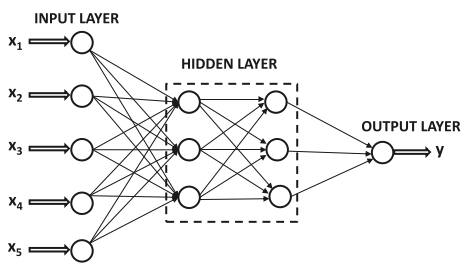
\includegraphics[width=\linewidth]{Figures/fig_ffnn_no_bias.png}
  \caption{No bias neurons}
  \label{fig:ffnn_wo_bias}
\end{subfigure}%
\hspace{0.5cm}
\begin{subfigure}[t]{.5\textwidth}
  %\centering
  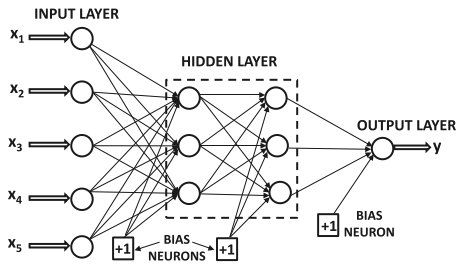
\includegraphics[width=\linewidth]{Figures/fig_ffnn_bias.png}
  \caption{With bias neurons}
  \label{fig:ffnn_w_bias}
\end{subfigure}
 \caption{Overview of a simple feed forward neural network architecture. Image extracted from a book~\protect\cite{DBLP:books/sp/Aggarwal18}} 
  \label{fig:whole_ffnn}
\end{figure}
% \begin{figure*}[h]
% \centering
%  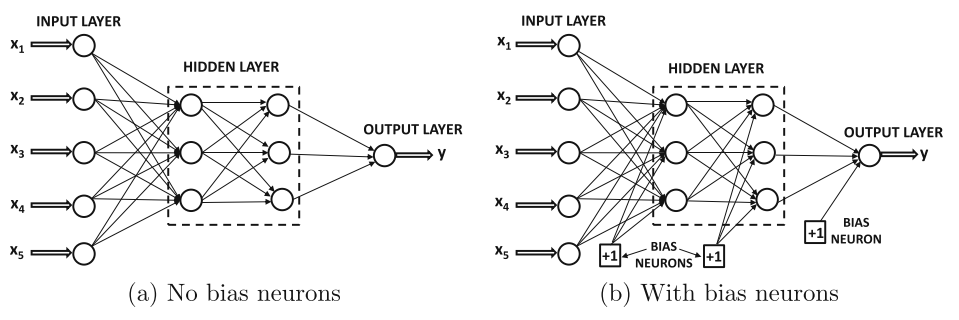
\includegraphics[width=\linewidth]{Figures/fig_ffnn.png}
%  \caption{Overview of a simple feed forward neural network architecture. Image extracted from a book~\protect\cite{DBLP:books/sp/Aggarwal18}.}
%  \label{fig:feed_forward_nn}
% \end{figure*}
%In this subsection simple feed forward neural networks (aka shallow neural networks) will be discussed. 

%The simple architecture of \textit{3-layer} feed forward neural network (with 2 hidden and output layer) and with/out bias is shown in Figure~\ref{fig:feed_forward_nn}. %Often the input layer is not counted, The reason of why input layer often not counted because it simply transmits the data without any computation is performed. 

The default architecture of feed forward neural networks (e.g., Figure~\ref{fig:ffnn_w_bias} ) contain a series of fully connected layers, i.e, each node in one layer is connected to nodes of the subsequent layer. For example, the Figure~\ref{fig:ffnn_w_bias} is a \textit{3-layer} (with 2 hidden and an output layer) neural network. The feed forward neural networks have standard architecture. Hence, once the number of layers, nodes in each layer and the loss function are defined then the rest of the architecture of the network is straight-forward.

In feed forward neural networks each connection i.e. \textit{edge} between a neuron in a layer and another neuron in the subsequent layer has a weight. Each neuron except the ones in the input layer, gets as an input of a sum of the multiplications of the inputs from the previous layer and their respective weights. Further, a bias value might also be added to this sum. Then, each neuron applies an activation function to produce an output. Note that the number of units in each layer is referred to as the dimensionality of that layer~\cite{DBLP:books/sp/Aggarwal18}.

Assume the input is \textit{d}-dimensional vector $\overline{X}$ where $\overline{X}=[x_1,x_2,...,x_d]$ and let $p_1$ denote the number of units in the first hidden layer. $W_1$ is a matrix such that $W_1 \in \mathbb{R}^{d\times p_1}$  and it contains the weights of the connections between the input layer and the first hidden layer. Similarly, the dimension of the weight matrices in the hidden layers determined by the number of neurons contained in that layers. Assume $W_r$ is a weight matrix between $r$th hidden layer and the $(r+1)$th hidden layer, then $W_r \in \mathbb{R}^{p_r\times p_{r+1}}$. Finally, assume the output layer contains $o$ nodes, then the final weight matrix is $W_{k+1}$ and $W_{k+1} \in \mathbb{R}^{p_k\times o}$. 

Given input $\overline{X}$ in order to produce the output $\bar{o}$ the following recursive equations~\cite{DBLP:books/sp/Aggarwal18} is used as follows:

\begin{align*}
& \bar{h}_1= \Phi (W_1^{T} \overline{X}) \\
& \bar{h}_{p+1}= \Phi (W_{p+1}^{T} \overline{h}_p), \forall p \in \{1,...,k-1\} \\
& \bar{o}=\Phi (W_{k+1}^{T} \overline{h}_k)
\end{align*}\\ \todo[color=green!40]{here explain the formulas e.g., input to hidden }
where $\bar{h}_1$ is the column vector of an output of the first hidden layer, similarly, $\overline{h}_{p+1}$ is a column vector of an output of ${(i+1)}^{th}$ layer,
%$p+1$ denotes the number units in  layer and the column representation of their output is $\overline{h}_{p+1}$. 
$\Phi$ is an activation function such as sigmoid, ReLU, etc.  

It is often the case that different layers of a network use different activation functions. For example, a simple feed forward neural network which is designed for a binary classification task, often uses ReLU in the hidden layers and the sigmoid for the output layer. It should be noted that all units in a layer use the same activation function. Further, depending on the application at hand (e.g., classification or dimensionality reduction), it is possible to vary the architecture of the neural network easily to allow multiple outputs.
%In a default architecture of feed forward neural network ReLU activation function is commonly used in hidden layers and for binary outputs sigmoid function is used in the last layer of the network. %In such an architecture another common activation functions for the hidden layers is ReLU and for binary outputs is sigmoid function. 
%softmax function outputs with cross-entropy loss for discrete prediction. 

The given equations above is the general formulation of the forward operation which aims to transform the given input feature vectors into the outputs. %After each forward operation or after a small patch of a forward operation the weight are updated. 
In other words, similar to perceptron algorithm, each input data is fed into the network one by one or in small batches in order to produce outputs. In perceptron the training process is straightforward because the
optimization is achieved by minimizing the heuristically motivated simple loss function. However, in a multi-layer neural network the loss function is much more sophisticated. The function is a composition of all the weights in each layer. The weight values are updated according to the error gradients. In order to compute the gradient of the composition function \textit{backpropagation} algorithm has been widely leveraged for training feed forward neural networks.
%The above equations are general formulation of the forward operation where the given input vectors are transformed into the outputs.
%element-wise fashion to their vector arguments.  some activation functions such as the softmax (which are typically used in the output layers) naturally have vector arguments
%The  arch is shown in Fig explain fig with bias 
%Sin it only transmits the data no computation is performed % of learning such a nn architecture.
%backpropagate’ the errors through the layers widely used Backpropagation is a %core method of learning such a nn architecture.
%backpropagate’ the errors through the layers
%widely used algorithm for training feed forward neural networks. 
Such training process mainly relies on the modification or update of weights and biases during the training process with backpropagation. In the following backpropagation algorithm is briefly explained and more details can be found in~\cite{DBLP:series/utcs/Skansi18}. 

%In other words, Backpropagation is widely used algorithm for training ffnn. %the learning process in the neurons is simply the modification or update of weights and biases during training with back propagation. 
First an error function $E(x)$ or cost function which measures the performance of the network is defined as follows\todo{check formulas}:% from other book with y hat
%formula where formulas has no number Introduction to deep learning
\begin{equation}
    E= \frac{1}{2}\sum_{n\in D} (y^{(n)}-\hat{y}^{(n)})^2
\end{equation}
where $n$ denotes the training sample, $y$ is the target for the training case $n$ and the $\hat{y}$ is the prediction, i.e., output of the model. The error function sums error across all the training samples, then the weights are updated accordingly. 

Based on backpropagation the derivative of error function $E$ is taken with respect to $w_i$:
\begin{equation}
    \frac{\partial E}{\partial w_i}=\frac{1}{2}\sum_{n} \frac{\partial y^{(n)}}{\partial w_i} \frac{dE^{(n)}}{y^{(n)}}
\end{equation}

The weight updates are proportional to the error derivations in all training samples and they are added together:
\begin{equation}
    \triangle w_i = - \eta \frac{\partial E}{\partial w_i} = \sum_{n} \eta x_i^{(n)} (y^{(n)} - \hat{y}^{(n)})
\end{equation}
%formula
The details of the derivatives are shown in~\cite{}
Finally, the wights are updated according to the formula below:
%formula page 94
\begin{equation}
   w_{update}= w_{old}-\eta \nabla E
\end{equation}
    
\subsection{Convolutional Neural Networks}
\label{subsec:CNNs}
Convolutional neural networks (CNNs) are specialized neural networks for processing grid-structured data, e.g., image data (2D grid), time series data (1D grid). The most distinctive feature of convolutional neural networks from other networks is the \textit{convolutional} layer. Typically, a traditional convolutional  network architecture contains at least one convolutional layer. 

In 1998, the first convolutional neural network \textit{LeNet-5} was developed by LeCun, Bottou, Bengio and Haffner. This network was trained with MNIST data which is a large dataset and contains binary images of handwritten digits. Thereafter, convolutional neural networks have been utilized in variety of applications. In 2011, convolutional neural networks demonstrated remarkable performance in an image-classification contest. After that convolutional neural networks gained significant attention, especially, in the field of image processing. Although they can be utilized with various type of data, the majority of the applications have been focused on image data. Some of the example of applications are image classification, image and video recognition, medical image analysis, etc.
%Although CNNs have been utilized in variety of applications since 1990s,

Although convolutional neural networks have been mostly utilized in the field of image processing, applying them for natural language processing tasks has also been  explored.In 2014,~\citeauthor{DBLP:conf/emnlp/Kim14} designed a relatively simple convolutional neural network architecture for a sentence classification task~\cite{DBLP:conf/emnlp/Kim14}\todo{check teh architecture and extnd this part}. Each input sentence first tokenized and the tokens are converted into a sentence matrix by utilizing Google pre-trained word vectors.\todo{heck this and cite} The model demonstrated strong empirical performance across several datasets. Today, the proposed model by Kim is still one of the most widely used baselines for sentence classification. After the publication of the paper by ~\cite{DBLP:conf/emnlp/Kim14}, convolutional networks draw significant attention from the natural language processing community. Several scientific literatures have been published in the similar direction~\cite{}.\todo{cite}

%until the adaption of a CNN architecture for a sentence classification task by~\cite{DBLP:conf/emnlp/Kim14}. %~\cite{DBLP:conf/emnlp/Kim14} utilizes word embeddings for  if you like you can extend this part
%Although CNNs have been utilized in variety of applications since 1990s, after the publication of the paper by ~\cite{DBLP:conf/emnlp/Kim14} CNNs gained significant attention for text classification task. The proposed architecture by Kim is relatively simple, i.e., 1-layer CNN yet demonstrated strong empirical performance across several datasets. Soon later several papers have been published in this direction~\cite{}.
%Today, the proposed model by Kim still the one of the most widely used supervised baselines for text classification. 

%Therefore, in this chapter first general architecture of convolutional neural networks where the input is image data and then application of convolutional neural networks to text categorization task have been described. 

% The general architecture of CNNs are explained in Section~\ref{subsec:CNNs}. CNNs have been used widely in the applications of image and video recognition, image classification, medical image analysis, etc. However, after ~\cite{DBLP:conf/emnlp/Kim14} proposed a CNN architecture for sentence classification, the model has gained significant attention among the NLP applications such as text categorization, sentiment analysis, etc. Considering that this thesis is about text categorization, here we explain the adaption of convolutional neural networks to text categorization task. 




%Unlike image data (usually 3 dimensional including colors), text data data can be represented with 2-dimentsional vectors. 



% \begin{figure*}[h]
% \centering
%  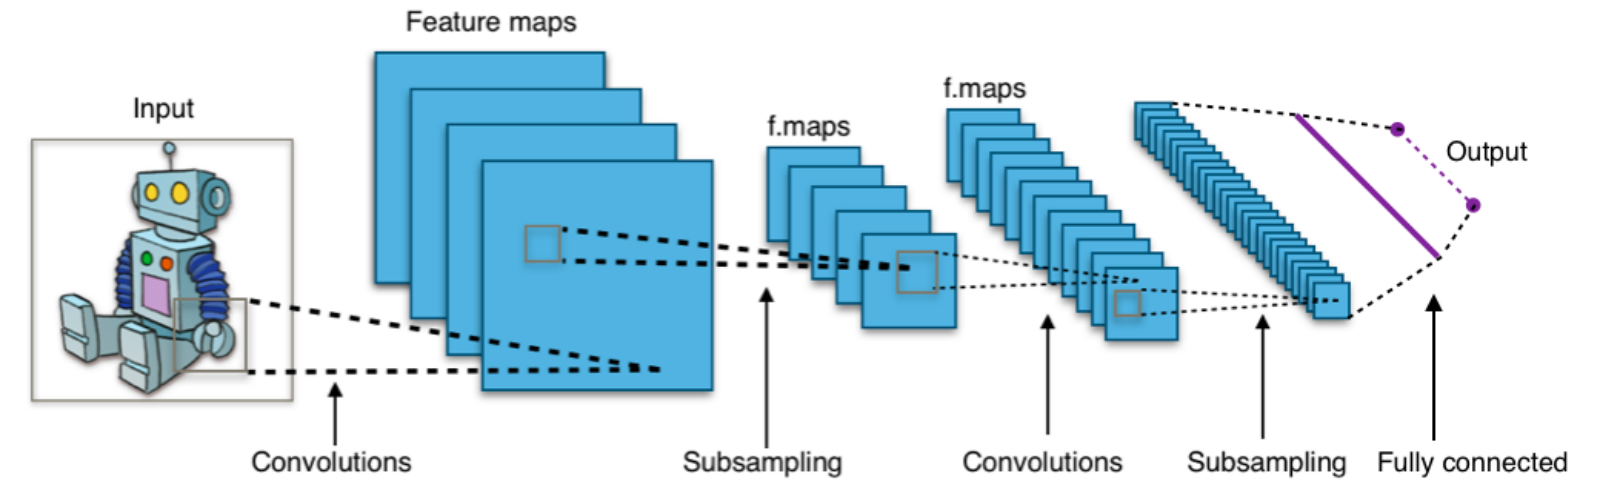
\includegraphics[width=\linewidth]{Figures/fig_cnn.png}
%  \caption{Overview of a simple convolutional neural network architecture.}
%  \label{fig:cnn}
% \end{figure*}
\begin{figure*}[h]
\centering
 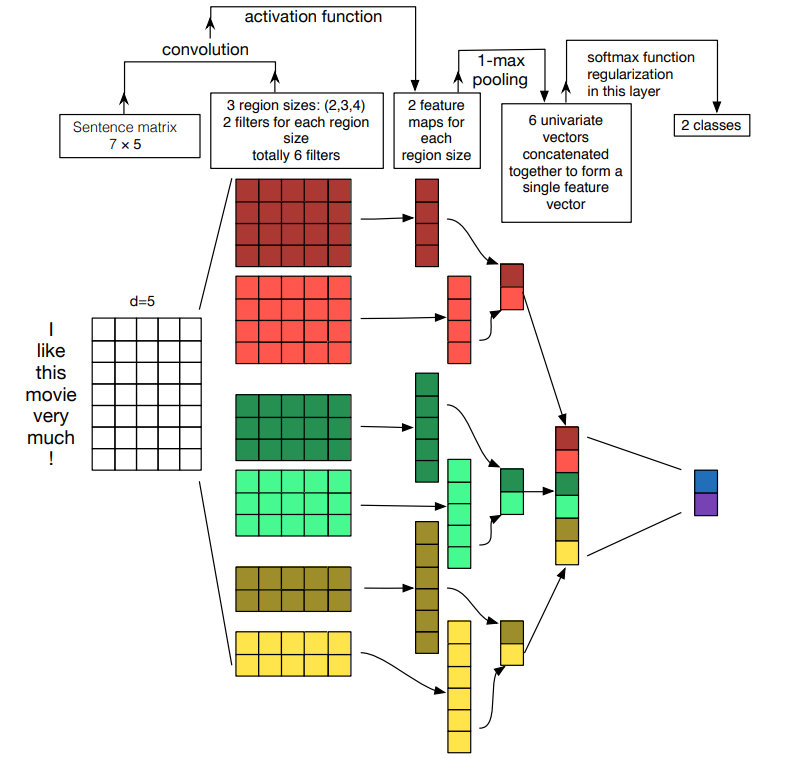
\includegraphics[width=\linewidth]{Figures/fig_cnn_for_text_cat.png}
 \caption{A CNN architecture for sentence classification. The image is extracted from~\protect\cite{DBLP:conf/ijcnlp/ZhangW17}.}
 \label{fig:cnn_text_cat}
\end{figure*}

The convolutional neural networks are similar to the traditional feed forward neural networks in the sense that the information moves in only forward direction, i.e, from an input layer to hidden layers and finally to an output layer. Figure~\ref{fig:cnn_text_cat} illustrates a  simple example of a convolutional neural network architecture for a sentence classification task. Unlike feed forward neural networks, which typically contain one type of a hidden layer i.e, fully connected layer, convolutional neural networks consist of different type of hidden layers.  The most common three type of layers which are contained in standard convolutional neural networks are \textit{convolution}, \textit{pooling},and \textit{ReLU} layer. ReLU is an activation layer which is similarly applied as in the traditional neural networks. Beside the aforementioned layers, the final layers of convolutional networks are often fully connected. The layer just before  the output layer is mapped to the output layer to produce the final output of a network. The  number of nodes in an output layer determined in an application specific way.   %  which maps given inputs into the set of output nodes. 

Before discussing the layers of convolutional neural networks, first, we briefly examine a general architecture of the network. The majority of the related literature has been focused on analyzing the model in an image classification setting where the input is image data. However, in this thesis our focus is text categorization, therefore, we discuss the model in the context of text categorization. %Therefore, we assume that our input is text data. 
Figure~\ref{fig:cnn_text_cat} illustrates a simple example of a convolutional neural network architecture which is designed for sentence classification. Given a piece of text, i.e., a sentence, the goal of the model is to assign a binary label to it. As already stated, convolutional neural networks accept grid-like structured data as an input, therefore, each input sentence converted into a sentence matrix. To that end, first, sentences are tokenized. The vector representation of tokens are utilized to form the sentence matrix. % and rows of the matrix are the vector representation of each token.
The rows of the matrix are the token vectors which can be obtained from e.g., a pre-trained Skip-gram model or any other word embedding model. Let $d$ denote the dimension of the word vectors and $s$ is the number of tokens present in a given sentence. Then, the dimensionality of the sentence matrix is $s\times d$. The value of $s$,\todo{ask about s} i.e., the number of tokens to be considered from an input sentence to form a sentence matrix is often predefined. Because, the dimension of the input matrix determines the number of neurons in the input layer. To define the value of $s$, often, the maximum length of the sentence in a given dataset is considered. Obviously, the length of the sentences in standard datasets may vary and thus the zero-\textit{padding} (cf. Section~\ref{subsec:padding}) strategy is used to equalize the dimension of the input matrices.  
Given a sentence matrix the next operation is the convolution which is performed via \textit{"filters"} or \textit{"kernels"}. The number and the size of the filters determined based on the application at hand. In Figure~\ref{fig:cnn_text_cat} there are 6 different filters with 3 different sizes. After the convolution operation the obtained feature maps have different dimensionalities. In order to induce them to a fixed length vector and reduce the dimensionality of the feature maps a max-pooling function is applied to each feature map independently.  
%extract a scalar from each feature map and induce them to a fixed length vector max-pooling function is applied.  
%based on the filter size and thus a pooling function is applied to each feature map to extract a scalar from each feature map and induce a fixed length vector.
Thereafter, those vectors are concatenated to form a single dense feature vector. To produce the outputs, softmax function is applied to this vector. It should be noted that the it is possible to feed the dense feature vector through a fully connected layers and then the output layer. The architectural design of the network can be easily altered based on the application at hand.\\
%can be fed through a fully connected layer and then a softmax function or directly to a softmax function. \\
 %or to a fully connected layer then to a softmax function to produce the outputs. 
In the next subsections the details of each layer is\todo{check grammer} discussed.  
%Given an input text the first step is tokenization. As it has already mentioned, convolutional neural networks accept grid-like structured data as an input, therefore, tokens are converted to a sentence matrix. 
%Hence, the input to the convolutional neural network is organized into a 2-dimensional grid structure and each grid value is referred to as \textit{pixels}. Each pixel corresponds to a spatial location within the image. Further, in order to encode the color i.e., red, green, and blue of each pixel multi dimensional array of values at each grid location is being used. Assume that given an image with 32 × 32 spatial dimensions and the depth is 3 , then the overall number of pixels in the image would be 32 × 32 × 3. Moreover, in convolutional neural networks filters or kernels often are organized into 3-dimensional structural units (see Fig. ) which are usually much smaller than those of the layer the filter is applied to. Further, the filter is usually square in terms of its spatial dimension and the depth of it is always same as the layer to which it is applied. 

%intensity of the three primary colors i.e., red, green, and blue then the 
\begin{figure*}[t]
\centering
 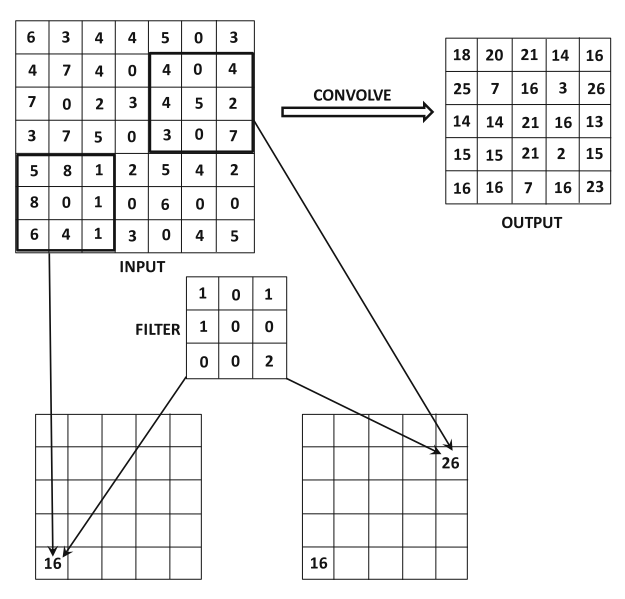
\includegraphics[width=\linewidth]{Figures/fig_cnn_convolution.png}
 \caption{An overview of a simple convolutional operation. The image is extracted from~\cite{DBLP:books/sp/Aggarwal18}}
 \label{fig:cnn_convolution}
\end{figure*}

\subsubsection{Convolution Operation}


The \textit{convolution operation} aims to produce a feature map from a given input and a kernel. Often, in a convolution layer the convolution is performed multiple times independently, and each time operation utilizes a different kernel.  

\todo{check (s)} The main idea is that the operation places the filter to each possible position of the input %(like a sliding window)  from left to the right and up to the down) 
and for each possible position dot product between the filter and the matching grid of the input is performed. To be able to perform such dot product the filter and the input should fully overlap.

Figure~\ref{fig:cnn_convolution} illustrates the general convolution operation. The layer size of the given example is $7\times7$ and the filter size is $3\times3$. The output matrix is the result of the convolution operation. There are two example numbers 16 and 26. Those numbers are the result of a dot product between the filter and the respective matching grid of the input. These values are obtained as follows:
\begin{align*}
& 5\times1+8\times1+1\times1+1\times2=16 \\
& 4\times1+4\times1+4\times1+7\times2=26
\end{align*}

When performing the convolution operation the filter should be alligned with the matrix in a way that no portion of the filter is sticking out from the borders of the matrix. The possible dot products defines the dimension of the next layer. Note that the size of the filters are determined based on the application at hand, e.g., for a sentence classification task given a sentence matrix where each row is a word vector, then it is reasonable to use filters with widths equal to dimension of the word vectors. Whereas for image processing the most common filter sizes are $3\times 3$ or $5\times 5$.  \\
The convolution operation for the depicted scenario in Figure~\ref{fig:cnn_text_cat} can be formalized as follows:
Given a filter which is parametrized by the weight matrix $w$. The width of the filter is $d$ and the height is $h$, then the $w$ will contain $h \cdot d$ parameters to be estimated. Let $A$ denote sentence matrix by $A \in \mathbb{R}^{s\times d}$ where $s$ is number of tokens to be considered to form the sentence matrix and $A[i:j]$ represents the sub-matrix of $A$ from row $i$ to row $j$. Then the output of the convolution operation $o\in \mathbb{R}^{s-h+1}$ is obtained by iteratively applying the filter on sub-matrices of $A$ as follows:\todo{add general formula}

\begin{equation}
o_i = w \cdot A \left[i:i + h -1\right]
\end{equation}
where $i = 1,. . ., s\num{-h}+1$, and $\cdot$ is the dot product between the sub-matrix and the filter. \\
%However, if we use image data then the convolution operation can be formalized as follows: Given a two-dimensional image  (or any two-dimensional )$A$ and two-dimensional filter  $K$ the convolution operation can be formalized as follows:
%Figure 8.1 or 8.2
%The formal definiation of the convolution operation is as folows:

% \begin{equation}
% \begin{split}
% h_{ijp}^{(q+1)} = \sum_{r=1}^{F_q}\sum_{s=1}^{F_q}  \sum_{k=1}^{d_q} w_{rsk}^{(p,q)}h_{i+r-1,j+s-1,k}^{(q)} \forall i \in \{1,...,L_q-F_q +1\}& \\
% \forall j \in \{1,...,B_q-F_q +1\}&\\
% \forall p \in \{1,...,d_{q+1}\}&
% \end{split}
% \end{equation}



The convolution operation relies on three important ideas that improves the performance of the model\todo{reference}:\\
\begin{itemize}
\item \ \textbf{Sparse interactions.} The size of the filters or kernels are often much smaller than the layers of which the filters are applied to. Therefore, the feature maps which are output of the convolution operations have much smaller size than the input layers. Consequently, fewer parameters need to be stored and processed and thus the efficiency is improved automatically. For example; an input of an image can have millions of pixels to be processed. However, with the help of kernels the meaningful features can be detected by utilizing only tens or hundreds of pixels~\cite{goodfellow2016deep}.\\
%output of the convolution operation produces one or more feature maps have much smaller size than the layer. In other words, after applying a convolution operation to a layer the output has  number of the parameters are reduced and thus fewer parameters need to be stored.
\item \ \textbf{Parameter sharing.}
As the name indicates parameter sharing refers using the same parameters in multiple operations. For example,  in a convolution operation, in order to produce a feature map, a kernel slides over an input of which the filter is applied to. In other words, the kernel visits every possible location of the input. However, instead of learning a parameter for each location/pixel (in case of image data) of the input, only one set of parameters, i.e., the kernel's parameters are learned.\\ %vs dense matrix multiplication
\item \ \textbf{Equivariant representations.} The idea of parameter sharing enables a layer to be equivariance to translations~\cite{goodfellow2016deep}. The functions $f(x)$ and $g(x)$ are considered to be equivariant to each other if  $g(f(x)) = f(g(x))$. For the sake of simplicity we give the following example~\cite{goodfellow2016deep}. Let $I$ be a function which gives the coordinates of a certain feature e.g., brightness of a given image. Let $g$ be a function such that $I^{'} = g(I)$ and $I^{'}(x,y)=I(x-1,y)$ which shifts the every pixel of $I$ to one unit right. Then, according to equivariant representations the output of the following two operations will be the same: (1) first applying the translation function $g$ to $I$ then applying convolution, (2) applying convolution $I^'$ and then applying $g$. 
\end{itemize}

\subsubsection{Padding} \label{subsec:padding}
The size of an output of a convolution operation is often smaller than the size of the layer which the operation is applied to. Such reduction of the size tend to cause lose of information and thus depending on the application it may not be desirable. This issue can be addressed by using \textit{padding} method. Figure~\ref{fig:cnn_padding} illustrates zero-padding operation. The basic idea of padding is before applying convolution operation, adding zero pixels all around the input. By doing so, it can be ensured that the input volume and output volume will have the same size spatially. Further, since the padded pixel values are zero they do not contribute to the final dot product values. We give the following example to explain the padding method clearly~\cite{goodfellow2016deep}. Given an input which has the size $32\times32\times1$ and the filter is of a size $5\times5\times1$. The zero padding is applied to an input according to the formula $(F-1)/2$ where $F$ is the width or height of a filter. According to the given example, $F$ is equal to 5. Given that $(5-1)/2=2$,  $2$ zeros are padded on all the sides of the image. As a result, first the size of the input increased from $32\times32\times1$ to $36\times36\times1$ and then after the convolution operation (with a filter size $3\times3\times1$) the size of the feature map is $32\times32\times1$ which is the same as the initial input.

%Increasing spatial height and width of the input volume with zero padding ensures that the input volume and output volume will have the same size spatially.


%To avoid such an issue one of the most common way is to use \textit{padding}. In padding operation, first extra added to (Fq \−1)\/2 pixels all around the borders of the feature map, then those pixel values are set to zero as shown in Figure... 

\begin{figure*}[h]
\centering
 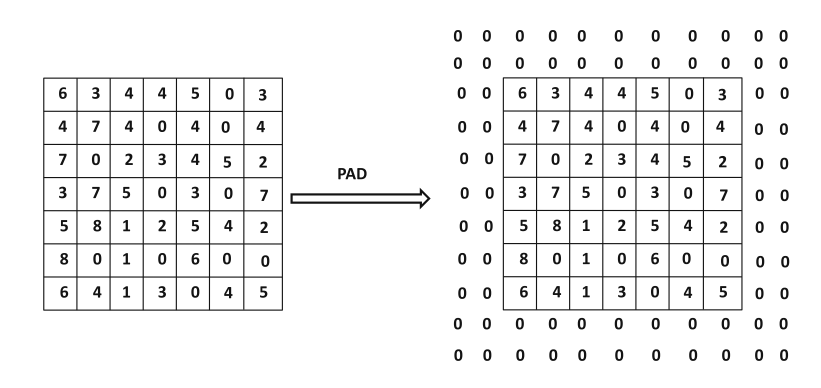
\includegraphics[width=\linewidth]{Figures/fig_cnn_padding.png}
 \caption{An overview of a simple convolutional neural network architecture. The image is extracted from~\cite{DBLP:books/sp/Aggarwal18}.}
 \label{fig:cnn_padding}
\end{figure*}
%The convolution operation reduces the size of the input volume by (Fq-1). Increasing spatial height and width of the input volume by (Fq-1) with zero padding ensures that the input volume and output volume will have the same size spatially. %As a result, the convolution operation is performed after pading the input the size of the  
\subsubsection{ReLU Layers}
The ReLU layers  basically responsible for applying the traditional ReLU activation function to a layer. More precisely, let $W_r$ such that  $W_r \in \mathbb{R}^{p_r\times p_{r+1}}$ to denote a parameter matrix between $r^{th}$ hidden layer and $(r+1)^{th}$ layer. The ReLU function is applied to each entry of $W_r$ to create the same size of a matrix $p_r\times p_{r+1}$ with thresholded values. Those values are then fed  into the next layer. The size of the input remains the same after applying the ReLU function. Moreover, often, this layer is not depicted in an architectural illustration of a typical convolutional network.  

In the previous years, other activation functions such as sigmoid and tanh were very popular. However, ~\cite{DBLP:conf/nips/KrizhevskySH12} has shown that usage of ReLU has many advantages in comparison to other activation functions. More precisely, ReLU improves the performance of a neural network in terms of speed and accuracy.  Hence, %Although there exist many other activation functions the 
ReLU is one the most commonly used activation functions, especially in convolutional neural networks. %There are two main reasons for this occurrence. The first one is the 
%The ReLU activation layer is similarly applied as in a traditional neural network. Often, ReLU layer is not explicitly depicted in architectural representation of the convolutional neural networks. For each of the Lq ×Bq ×dq values in a layer, the ReLU activation function is applied to it to create Lq ×Bq ×dq thereshold values. The dimension of the ReLU applied layer remains the same. Finally, these threshold values are passed to the next layer. %ReLU has a lo of advantages than the other activation functions
\subsubsection{Pooling Layers}\todo{update the picture}
The poling operation transforms the input into a smaller but more compact representation and it is applied in every convolutional layer. Figure~\ref{fig:cnn_pooling} illustrates an example of a pooling operation. The pooling layer takes a pool size such that $P_q \times P_q$. In the example the size of the pool is $3\times3$ and the input has the size $7\times7$. The pooling operation scans the input with a square regions of size $3\times3$. Then for each region maximum of these values is returned to form the output of the pooling operation. This entire operation is called as max pooling.
%The pooling operation works on a small square regions of size Pq x Pq. The pooling operation is performed at the level of each activation map and produces another layer with the same depth. For each square region of size Pq x Pq in an activation map the maximum values are returned and this operation is refered as max pooling. The pooling operation reduces the spatial dimension of the activation map. 
\begin{figure*}[h]
\centering
 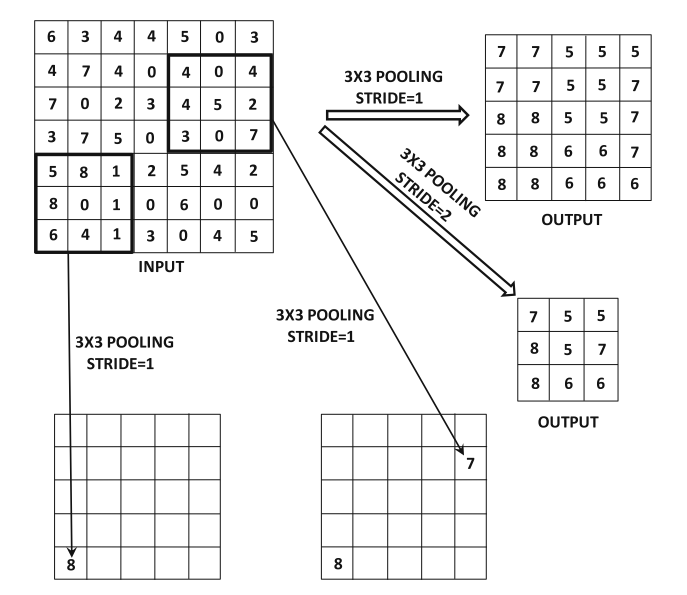
\includegraphics[width=\linewidth]{Figures/fig_cnn_pooling.png}
 \caption{An overview of a simple convolutional neural network architecture. The image is extracted from~\cite{DBLP:books/sp/Aggarwal18}.}
 \label{fig:cnn_pooling}
\end{figure*}
There are also other type of poolings such as average-pooling. However, they are rarely used. 
\subsubsection{Fully Connected Layers}
The fully connected layers are similar to the traditional feed forward networks. Depending on the application at hand the number of fully connected layers can be specified. However, often it is common to use more than one fully connected layer in order to increase the performance of the network. The aforementioned layers, i.e., convolutional and pooling layers process grid-like structured data. However, the feed forward neural networks designed to process inputs in form of a column vector. Therefore, before feeding an input to a fully connected layer, the input is flattened as shown in Figure\todo{figure flattening}.
%Before feeding the layer just before the fully connceted layer is flattened . 
Thereafter, the flattened vector is fed to the fully connected layer. The last layer of the connected layer fed to the output layer. 
\begin{figure*}[h]
\centering
 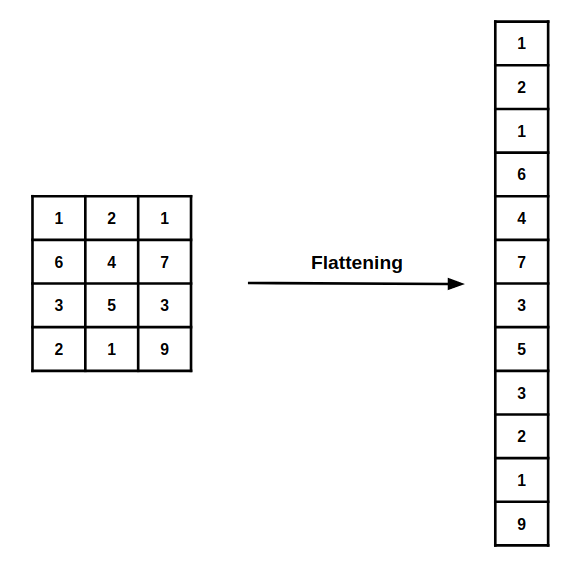
\includegraphics[height=5cm,width=5cm]{Figures/fig_cnn_flattening.png}
 \caption{An overview of a flattening operation.}
 \label{fig:cnn_flattening}
\end{figure*}
\todo{training a cnn mention} 
%The final spatial layer is connected to a first fully connected layer. This layer is exactly the same as traditional ffnns. Depending on the application at hand the number of the fully connected layers and the activation function output layer  
\subsection{Recurrent Neural Networks}
The aforementioned networks in the previous sections, i.e., feed forward and convolutional neural networks are designed to process data whose attributes do not depend on each other. However, certain data types like text or time  series data sequentially depends on each other. Obviously,  text data can be processed by a simple feed forward neural network. However, the sequential information of the words is not taken into account by such a network. Recurrent neural networks are specialized for processing sequential data, and they are most commonly used with text data. 

Text data often processed by the approaches that rely on  bag-of-words representations for the categorization task. 
%The approaches that utilize text data for categorization often rely on the bag of words representations. 
Such methods ignore the sequential information of the words. Bag-of-words representations may work well for the classification task. However, for more sophisticated tasks, e.g, machine translation, sentiment analysis, the ordering of the words might be a critical feature. Therefore, in such tasks recurrent neural networks have been utilized successfully. 

Recurrent neural networks have simple architecture which is derived from conventional feed forward neural networks by adding \textit{recurrent} connections on hidden layers. Although the recurrent networks can be used almost with any sequential data, its application in the text domain is the most common. In the following we give examples of applications that commonly utilize recurrent neural networks~\cite{DBLP:books/sp/Aggarwal18}:\\
\begin{enumerate}
\item \textbf{Language models.} Given a set of history of words with their sequential information language models aim to predict the next word in that sequence. This is a typical scenario of standard language models which find their application in various areas of text mining and information retrieval.\\

\item \textbf{Auto regressive analysis.} Auto regressive analysis tasks aim to learn next element of a given real-valued time-series.\\

\item \textbf{Machine translation.} Given a sentence as an input machine translation aims to translate the sentence into desired language. In such a scenario the input is a sentence and the output is a sentence as well.\\

\item \textbf{Text categorization.} Text categorization aims to assign one or more predefined categories to a given sentence. In the case of text categorization, the input is a pieces of text and the output is a vector of class probabilities. \\

\end{enumerate}
%The given examples above are only some of the most prominent applications of the recurrent neural networks. 
\begin{figure*}[h]
\centering
 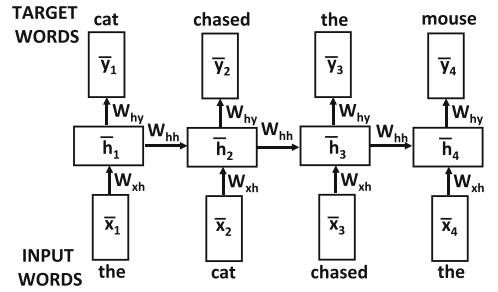
\includegraphics[height=5cm, width=10cm]{Figures/fig_rnn.png}
 \caption{Overview of a simple recurrent neural network architecture which is suited to language modeling. The image is extracted from~\cite{DBLP:books/sp/Aggarwal18}}
 \label{fig:rnn}
\end{figure*}


The simple recurrent network representation is shown in Figure~\ref{fig:rnn}. This architecture is particularly designed for language modeling, which aims to predict a next word, given the history of the words. The main characteristic of the network is that presence of shared weight matrices, i.e., $W_{xh}, W_{hh}, W_{hy}$ in the temporal layers of the network. Each time-stamp, i.e, the position in the sequence (starts at 0 (or 1), and increases by 1) has an input,
output, and hidden unit. Each word from a given sequence, first, one-hot encoded and then is fed one at a time to the neural network. In other words, each word is fed to the network at the relevant time-stamps.
%this temporal process is same as feeding each word to the inputs  %A time-stamp refers to a position of a word in the sequence. 
In the given example of a language model the output is a vector of probabilities predicted for the next word. %finish

Given an input vector at time \textit{t} (e.g., one hot encoded $t^{th}$ word of the sequence) is $\overline{x}_t$, the hidden state is $\overline{h}_t$ and the output $\overline{y}_t$ which is the predicted probabilities of the $(t+1)^{th}$ word. The hidden state can be formulated as follows:
    \begin{equation}
    \label{eq:rnn_hiddenlayer}
    \overline{h}_t = f(\overline{h}_{t-1},\overline{x}_{t})
\end{equation}
where $\overline{h}_{(t-1)}$ is the hidden vector at time $\textit (t-1)$, and input $\overline{x}_t$ and output $\overline{y}_t$ are $d$-dimensional vector of a vocabulary of size $d$. Further, the function $f$ utilizes weight matrices and activation functions to compute the all the hidden states. Although each hidden state is updated at each time stamp, the same weight values remain the same over the all time-stamps for a given sequential elements. 
%To formulate the entire training processes we consider the simple case in Figure. The hidden state at time \textit{t} as follows:
%formula 7.1where xt is the input vector and ht-1 is t hidden vector at tme (\textit{t}-1). 
Equation~\ref{eq:rnn_hiddenlayer} can be expanded to include also the output  as follows:
 \begin{equation}
 \begin{aligned}
    \label{eq:rnn_hiddenlayer}
    &\overline{h}_t = tanh(\overline{W}_{xh}\overline{x}_{t} +  \overline{W}_{hh}\overline{h}_{t-1})\\
    &\overline{y}_t = W_{hy}\overline{h}_{t}
\end{aligned}
\end{equation}
where "tanh" denotes an activation function, $W_{xh}$ is input-hidden matrix and $W_{hh}$ is a hidden-hidden matrix (cf. Figure~\ref{fig:rnn}), and $\overline{y}_t$ is an output.  
%formula 7.2
%Here the “tanh” notation is used to denote an activation function, depending on the application at hand different activation functions can be used such as sigmoid,...

%The hidden state of the network changes after the input of the each word in the sequence and the weight matrices in different layers are shared to ensure that the same activation function is used at each time-stamp. The particular architecture shown is suited to language modeling. The figure is  language modeling by predicting the next word given the previouse history of words. One hot coding of words are fed one at a time in Fig. relavent time stamp
The given architecture in Figure~\ref{fig:rnn} can easily be modified in order to be employed for other applications. In other words, depending on the application at hand it is possible that input or outputs units to be missing. Figure~\ref{fig:rnn_missing_input_output} illustrates different variations of recurrent networks for different applications. For example, for a sentiment analysis task which is a special type of a text categorization application the input is a sequential data and the output corresponds to the class of the given sequence. 
\begin{figure*}[h]
\centering
 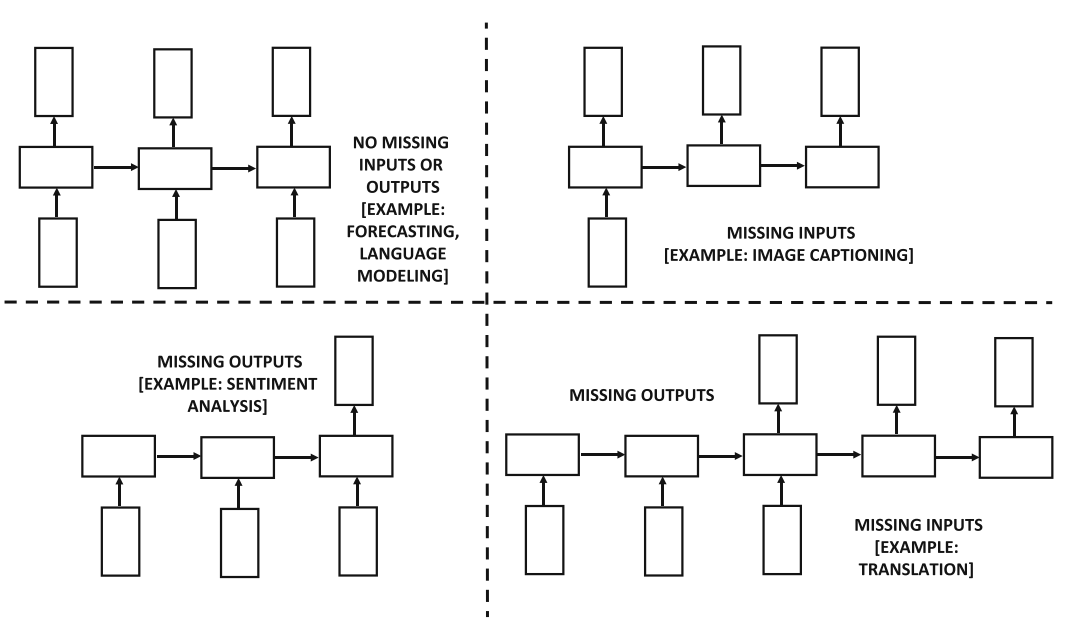
\includegraphics[width=\linewidth]{Figures/fig_rnn_missing_input_output.png}
 \caption{Examples of different recurrent neural network architectures. The image is extracted from~\cite{DBLP:books/sp/Aggarwal18}.}
 \label{fig:rnn_missing_input_output}
\end{figure*}


%Example of a sentiment analysis architecture which is a special type of a text categorization application is shown in Fig . In sequence classification application such as sentiment analysis we need only one output label which corresponds to the class of the given sequence. 
\subsection{Neural Language Models}
The idea of enabling intelligent systems to understand natural language has been a goal of various fields in Artificial Intelligence. Such systems require natural language data to be represented in a certain format to be able to process it. 
%Hence, it is crucial to represent text data in a form that the machine learning algorithms can process it automatically.  %require a certain representation of text data to be able to process and make sense of it. 
The raw representation of the data which consist of set of words cannot be directly processed by the machine learning systems~\cite{srinivasan2017guide}. One of the common ways to represent text is %through
in a form of a sparse and high dimensional discrete vector. There are several methods e.g., one hot encoding, bag-of-words, etc. can be exploited to obtain such text representations. However, such representation models have two main disadvantages. First, the dimension of the vectors is high which determined by the number of words present in vocabulary.  Secondly, to generate text vectors the semantic relation between the words are not taken into account.  Besides, such models often lead to inaccurate results on new and rare words. 

%The Vector Space Model (VSM) is one of the most successful and widely used approach to represent text documents~\cite{survey_word_embeddings}. The vector space model originally deveoped for an infomration retriaval system. There are various ways of building VSMs such as ... 
Motivated by the aforementioned challenges of text representations, \textit{word embedding} models have emerged as an important field of research in many NLP tasks~\cite{survey_word_embeddings}. Word embedding models aim to generate low dimensional vector representation of words or phrases by preserving syntactic and semantic relationships. The models are trained to learn the vector representation of words in a way that semantically similar words have similar representations. Hence, such words are placed %models are trained to place semantically similar words 
 close to each other in the vector space. %For example, semantically similar words are placed close to each other in the vector space. 
%For example, vector of "Berlin" and "Paris" located close to each other as they ca
%which is one of the most prominent word embedding models 
\begin{figure*}[t]
 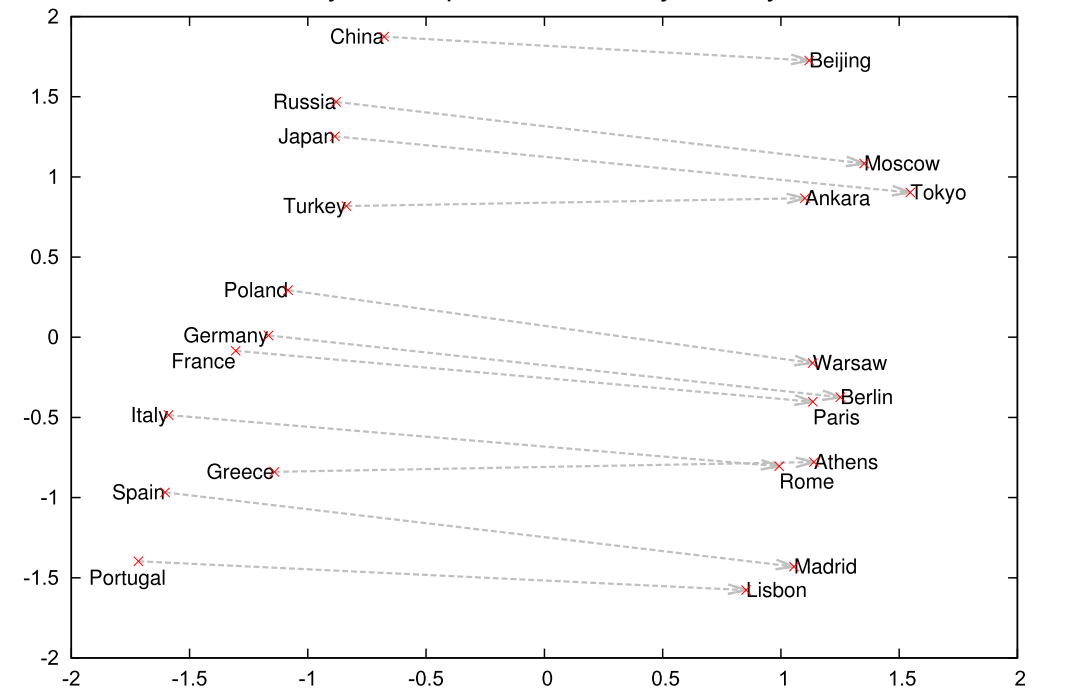
\includegraphics[width=\linewidth]{Figures/fig_word_vec_contries_capitals.png}
 \centering
 \caption{Two dimensional projection of Skip-gram vectors of countries and their capitals. Image extracted from~\protect\cite{DBLP:conf/nips/MikolovSCCD13}.}
 \label{fig:countries_capitals}
\end{figure*} 

Figure~\ref{fig:countries_capitals} illustrates an example of two dimensional projection of word vectors from a pre-trained word embedding model called Skip-gram~\cite{DBLP:conf/nips/MikolovSCCD13}. The capital cities e.g., "Berlin", "Paris", "Athens", etc. and countries e.g., "Germany" and "France", "Greece", are grouped successfully. Further, the location of the vectors reflect the implicit relationship, between them. Moreover, as Figure~\ref{fig:countries_capitals} shows that the distances between countries and their capital cities are approximately same. For example, vector("Paris") is the most closest word vector to the calculation of vector("Madrid") - vector("Spain") + vector("France") than any other word vector in the corpus~\cite{DBLP:conf/nips/MikolovSCCD13}. Another prominent example is in order to find  a word that is similar to "woman" in the same sense as "king" is similar to "man", a simple algebraic operation can be performed as vector("King") - vector("Man") + vector("Woman"), and the obtained result is a word vector of "Queen".
%here there was something

Word embedding models have been extensively leveraged in variety of natural language processing tasks, e.g., text classification, question answering, machine translation, semantic analysis. Moreover, it is also possible to leverage word vectors from embedding models to simply construct document vectors. Subsequently, the generated document vectors can also be utilized in wide range of natural language processing tasks such as query specific document ranking, document similarity calculation, document classification.
%word vectors from embedding models can be leveraged to simply construct text or document vectors. The generated document vectors can also be utilized in wide range of natural language processing tasks.% such as document classification, question answering, sentiment analysis, etc. 

Beside word embedding models, there is a considerable research body on \textit{document embedding} models which aim to generate the distributed representation of texts, i.e., documents, paragraphs, sentences. The basic idea of these models is that utilizing context word of documents to construct document vectors. \\
In the following, we give an overview of the most prominent word and document embedding models: \\
%Beside word embedding models, \textit{document embedding} models are proposed to generate the distributed representation of texts, i.e., documents, paragraphs, sentences. 
\begin{itemize}

\item \textbf{Skip-gram~\cite{DBLP:journals/corr/abs-1301-3781}.} The Skip-gram model learns the low dimensional representation of words while capturing syntactic and semantic word relationships from a given large corpus. The word vectors are computed by leveraging 2-layer simple feed forward neural networks. Training Skip-gram is very efficient, i.e., depending on the size of the corpus and the parameters it can only take a couple of hours. Moreover, the model can be easily adapted to obtain domain specific word or phrase representations. For example, for a patent classification task, the word vectors can be generated by training the model with a relevant large patent text corpus.
It should be noted that the Skip-gram model designed to be trained in an unsupervised manner.
\begin{figure*}[h]
\centering
 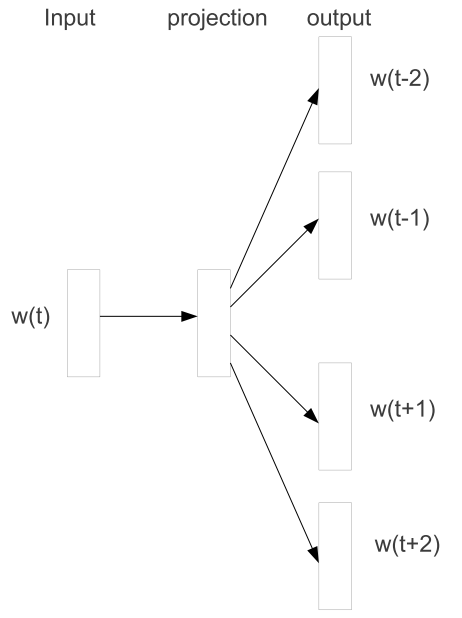
\includegraphics[height=4cm,width=4cm]{Figures/fig_skip_gram.png}
 \caption{Overview of Skip-gram model architecture. The image is extracted from~\protect\cite{DBLP:journals/corr/abs-1301-3781}.}
 \label{fig:skip_gram}
\end{figure*} 


Figure~\ref{fig:skip_gram} depicts the overview of Skip-gram model. For the sake of simplicity let $w(t-2),  w(t-1), w(t),  w(t+1), w(t+2)$ be a sequence of words from a given corpus. The basic idea of the model is given a word  $w(t)$ from a sequence, the model tries to predict the  probability for every word in the vocabulary of being the nearby word of $w(t)$, i.e., surrounding context word. According to Figure~\ref{fig:skip_gram}, $w(t)$ is a center word and its surrounding context words are $w(t-2), w(t-1), w(t+1), w(t+2)$. The number of surrounding context words for each center word is determined by a parameter called \textit{window size}. In this example the window size is equal to two as there are two left and two right context words for $w(t)$. 
%Ideally, the actual nearby words should have the higher probability than the other 

The goal of training Skip-gram model is to compute word vectors that are useful for predicting the surrounding words of a given center word. Then the objective of Skip-gram model is to maximize average log probability of a given sequence of words $w_1, w_2, w_3, ..., w_T$ as follows: 

\begin{equation}
\frac{1}{T}\sum_{t=1}^{T}\sum_{-c \leq j\leq c, j\neq0 } \textrm{log} p(w_{t+1}|w_{t})
\end{equation}
where $c$ is the size of the training context and specified with a window size. The bigger the window size is more the training samples are. \\
The probability $p(w_{t+1}|w_{t})$ defined by using softmax function: 
\begin{equation}
p(w_{O}|w_{I})=\frac{exp({v^{'}_{w_O}}^{T} {v}_{w_{I}})}{\sum\limits_{w=1}^{W} exp({v^{'}_w}^{T} {v}_{w_{I}})}
\end{equation}
where $v_w$ and $v'_w$ are input and output vector representation of $w$, and $W$ is the number of entire words in the vocabulary. Computing such an equation for each training sample is a very expensive task. Therefore, instead of calculating full softmax, hierarchical softmax which is computationally much more efficient is being used. Unlike softmax which evaluates $|W|$ output nodes to find the probability distribution, hierarchical softmax evaluates only approximately $\textrm{log}_2(W)$ nodes. The output layer is represented as a binary tree in hierarchical softmax. Each leaf node corresponds to a word $w$, $w \in W$. Each node in the tree represents relative probability of its child nodes. The hierarchical softmax defined as follows:

\begin{equation}
\displaystyle P(w|w_I) \prod_{j=1}^{L(w)-1} \sigma([n(w,j+1)=ch(n(w,j))]\cdot {v^{'}_{n(w,j)}}^{T} {v}_{w_{I}} )  
\end{equation}
where $n(w,j)$ is $j$-th node on the path from the root to $w$, $L(w)$ is the length of this path and $\sigma(x)=1/(1+exp(-x))$. Given the equation of hierarchical softmax the cost of computing $P(w|w_I)$ is on average not greater than $\textrm{log}W$.\\

Furthermore, the authors adapt Noise Contrastive Estimation (NCE)~\cite{cite} method as an alternative to the hierarchical softmax. Noise contrastive estimation is based on the idea that an ideal model should be capable of differentiating data from the noise through logistic regression model. Then for the Skip-gram model given  $P(w_O|w_I)$ the goal is to  distinguish between the target word $w_O$ and the negative samples which are drawn randomly. For each data sample there are $k$ negative samples. Then the objective of negative sampling defined as follows: 
\begin{equation}
 \textrm{log}\sigma({v^{'}_{w_O}}^{T} {v}_{w_{I}} )+ \sum_{i=1 }\mathbb{E}_{w_i\sim P_n(w)}\left[ \textrm{log}\sigma({- v^{'}_{w_O}}^{T} {v}_{w_{I}} ) \right] 
\end{equation}
where $P_n(w)$ is noise distribution from which the negative samples are drawn. $P_n(w)$ is a parameter and the authors show that the uniform distribution of it performs the best for several tasks.

The Skip-gram model requires large corpora for learning the vector representation of words, and obviously, the frequency of words has an impact on the quality of the vectors. In a very large corpora, usually the most frequent words are the least informative words (e.g., "the", "a", "an", "up"). To address this problem a simple subsampling approach has been defined as:
\begin{equation}
P(w_i)=1-\sqrt{\frac{t}{f(w_i)} }
\end{equation}
where $f(w_i)$ is the frequency of the word $w_i$ and $t$ is a chosen threshold, around $10^{-5}$. 

Overall, the Skip-gram model has been the base of many embedding models such as DeepWalk, node2vec, doc2vec etc. In addition, it is still one of the most standard baselines for many word, document and network embedding models.\\\todo{here you can explain word2vec model in 2 variations, i.e, skip-gram and cbow.}
% two-layer neural networks
%look at the words nearby and pick one at random. The network is going to tell us the probability for every word in our vocabulary of being the “nearby word” that we chose.

% and CBOW


\item \textbf{Doc2vec~\cite{DBLP:conf/icml/LeM14}.}
Doc2vec model extends Skip-gram model in order to obtain latent representation of texts  i.e., sentences, paragraphs, documents. Unlike Skip-gram which learns only the vector representation of words from a large corpora, doc2vec learns vector representation of words as well as documents (in which the words present). Doc2Vec is an unsupervised algorithm which is trained to be useful for predicting the words in documents to learn the document representations. Therefore, semantically similar documents or documents that share many common words expected to be located close to each other in the common vector space. 
\begin{figure*}[h]
\centering
 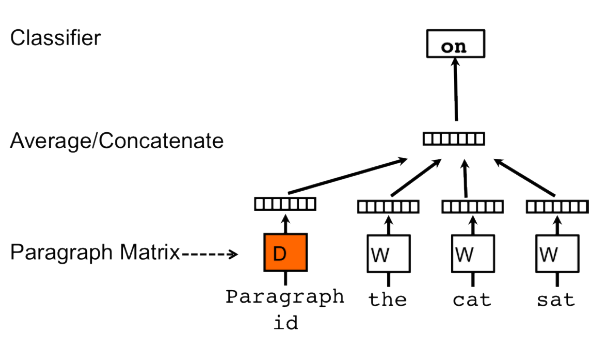
\includegraphics[height=5cm,width=8cm]{Figures/fig_doc2vec.png}
 \caption{Overview of doc2vec model architecture. The image is extracted from~\protect\cite{DBLP:conf/icml/LeM14}.}
 \label{fig:doc2vec}
\end{figure*} 
Figure~\ref{fig:doc2vec} illustrates the overview of doc2vec architecture. The document vector $D$ is concatenated (or averaged) with the word vectors $W$ from the document, then the model predicts the following word from the given context.

The model is inspired by the Skip-gram architecture, which is trained to predict a word from given context words. Similar to Skip-gram, the doc2vec model is also trained to predict next word from a given context information. However, in doc2vec the input is not only words but also a document vector which is treated similar as the word vectors. Every word and document from the given corpora mapped to unique vector. After the training, word and document vectors can be used in a wide range of natural language processing task such as text classification, question answering, text summarization etc. Since the architecture of doc2vec is very similar to Skip-gram, we do not discuss the technical details here. \\   

%\item \textbf{ELMo.}\\
\item \textbf{PTE~\cite{PTE}.} PTE aims to learn distributed representation of texts in a semi-supervised manner. It leverages both labeled and unlabeled data to learn the representation of documents. Further, unlike other embedding models such as Skip-gram which do not use any labeled data and generalizable for a variety of tasks, PTE designed to be utilized by a particular task.  More precisely, the obtained vector representations from PTE are easily fine tuned for a certain task with a set of labeled dataset. The general workflow of PTE is shown in Figure~\ref{fig:PTE}.\\
\vspace{0.1cm}
\begin{figure*}[h]
 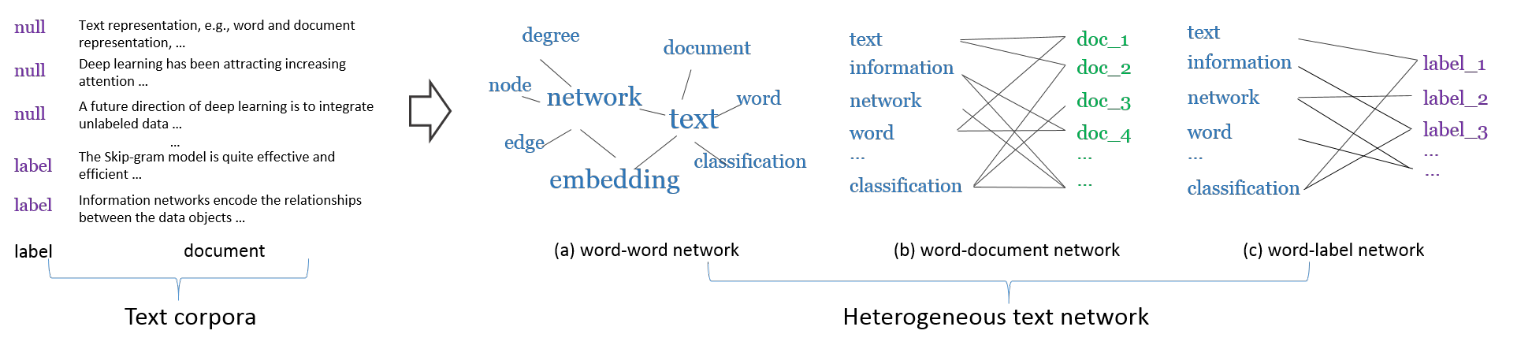
\includegraphics[width=\linewidth]{Figures/fig_PTE.png}
 \caption{An overview of converting text corpora to heterogeneous text network. The image is extracted from~\protect\cite{PTE}.}
 \label{fig:PTE}
\end{figure*} \\
Given a large text corpora PTE first encodes the different co-occurrence information  between words-words, words-documents and words-labels. 
\begin{itemize}
  \item Word-word network (cf. Figure~\ref{fig:PTE}a) captures the co-occurrence of words in the same local context. The weight of each edge of the network determined by the number of times that two word co-occur in the context windows.\\
  
  \item Word-document network (see Figure~\ref{fig:PTE}b) encodes the co-occurrence information of words in documents. The weight of an edges between a word and document defined by the number of times the word appears in the document. \\
  
  \item Word-label (cf. Figure~\ref{fig:PTE}c) network captures the information of category level word co-occurrences. The weight between the word $w_{i}$ and category word $c_{j}$ is $w_{ij}$ which is defined as: $w_{ij} = \sum_{(d:l_{d}=j)} {n_{di}}$ where $l{d}$ is a class label of document $d$ and $n_{di}$ is term frequency of word $v_{i}$. \\
  
  \item The combination of word-word, word-document, and word-label networks constitutes the heterogeneous text network.  \\
  
\end{itemize}

The heterogeneous text network is being exploited by PTE to learn the latent representation of words while preserving the second order proximity (cf. Section~\ref{subsec:network_embedding_models}).

The overall heterogeneous network consists of three homogeneous networks, i.e., the word-word, word-document and word-label networks. %PTE~\cite{PTE}, to embed each of these networks, aims to capture the second order proximity~\cite{tang2015line}.
To model the second-order proximity of a homogeneous network, for each edge $(v_i,v_j)$, the conditional probability $p(v_{j}|v_{i})$ is defined as follows~\cite{LINE}: 
\begin{equation}
%p(v_{j}|v_{i})=\frac{exp(-\vec{u}_{j}^{T}\cdot\vec{u}_{i})}{\sum\limits_{k=1}^{|V|} exp(-\vec{u}_{k}^{T}\cdot\vec{u}_{i})}\,,
p(v_{j}|v_{i})=\frac{exp(-\vec{u}_{j}^{T}\cdot\vec{u}_{i})}{\sum\limits_{v_k\in V} exp(-\vec{u}_{k}^{T}\cdot\vec{u}_{i})}\,,
%\raisepunct{,}
%p_{1}(v_{j}|v_{i})=\frac{exp(-\vec{u}_{i}^{T}.\vec{u}_{j})}{\sum_{k=1}^{V}exp(-\vec{u}_{i}^{T}.\vec{u}_{j})}
\end{equation}
where $V$ is the set of vertices connected with $v_i$ in the network, $\vec{u}_{i}$, $\vec{u}_{j}$ and $\vec{u}_{k}$ are the vectors of vertices $v_i$, $v_j$ and $v_k$, respectively. The empirical probability of $p(v_{j}|v_{i})$ can be defined as $\hat{p}(v_j|v_i)=\frac{w_{ij}}{d_i}$, where $d_i$ is the out-degree of $v_i$ and $w_{ij}$ is the weight of the edge $(v_i,v_j)$.

In order to preserve the second-order proximity, the conditional distribution $p(v_{j}|v_{i})$ is made close to $\hat{p}(v_{j}|v_{i})$ based on the KL-divergence over the entire set of vertices in the network, such that the model minimizes the following objective function:
\begin{equation}\label{optimizationHomo}
O=-\sum_{(v_i,v_j) \in E}w_{ij} \textrm{log} \,(p(v_{j}|v_{i}))\,,
\end{equation}

The embedding of the individual word-word, word-document and word-label networks are learned simultaneously by minimizing the following objective function:
% $O={O}_{ee}+{O}_{ec}$ .
 \begin{equation}\label{optimizationHet}
 O_{pte}={O}_{ww}+{O}_{wd}+{O}_{wl}\,,
 \end{equation}

where ${O}_{ww}$, ${O}_{wd}$ and ${O}_{wl}$ are the objective functions defined in Equation~(\ref{optimizationHomo}) for the homogeneous word-word, word-document and word-label networks, respectively. 
To optimize the objective function in Equation~(\ref{optimizationHet}), the edges are firstly collected from these three homogeneous networks as three sets, one for word-word edges, one for word-document edges and the other for word-label edges, and then in each training iteration, edges are sampled from each set to update the model. Readers can refer to~\cite{PTE,LINE}, for the detailed optimization process.

Once the word vectors are learned then the  representation of an arbitrary piece of text i.e., words $w_1, w_2, w_3,..., w_n$ present in text $d$ is simply inferred as the average of the word representations as follows:

\begin{equation}
\vec d= \frac{1}{n}\sum_{i=1}^{n}\vec u_{i}.
\end{equation}
\\
\item \textbf{BERT~\cite{DBLP:conf/naacl/DevlinCLT19}.} Bidirectional Encoder Representations from Transformers (BERT) is a language representation model which utilizes both jointly right and left context in all layers to pretrain deep bidirectional representations. The pretrained model then can be easily fine tuned to create language representation model for wide range natural language processing tasks. The technical implementation of BERT almost identical to the previous study by .... therefore, here we skip the technical details of the model.
The framework of BERT is shown in Figure~\ref{fig:bert}.
\vspace{0.3cm}
\begin{figure*}[h]
\centering
 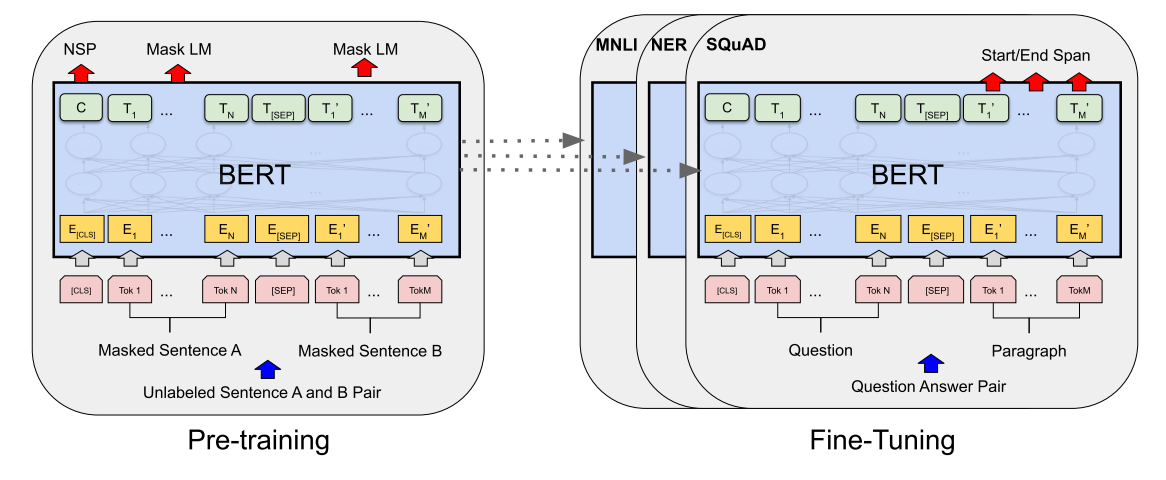
\includegraphics[width=\linewidth]{Figures/fig_BERT.png}
 \caption{An overview of BERT architecture. The image is extracted from~\protect\cite{DBLP:conf/naacl/DevlinCLT19}.}
 \label{fig:bert}
\end{figure*} 

BERT framework consists of two main steps (cf. Figure~\ref{fig:bert}) namely, pre-training and fine-tuning. Input to BERT is sequence of words which can be a single sentence or a pair of sentences. The first token of every input is always a special token ([CLS]) and the pair of sentences are separated by another special token ([SEP]). The input embedding of each token denoted as $E$ and the final hidden vector for the $i^{th}$ input token as $T_i$. \\
During the pre-training phase which is illustrated left part of Figure~\ref{fig:bert}, model is trained with two unsupervised tasks, namely, masked language modeling and next sentence prediction.
Masked language model task randomly masks some tokens of the input, then predicts those masked tokens. In this task, the final hidden vectors of masked tokens are fed into an output softmax over the vocabulary. Overall, the model tries to predict the masked inputs instead of an entire input.\\
The second task of pre-training is binarized next sentence prediction (NSP). The goal of the task is to train the model to learn the relationship between two sentences. The dataset for this task is easily generated from a given corpus.
%In order to train the model, the dataset generation phrase is straightforward. 
Given a sentence A and if the sentence B is the actual next sentence that follows A then labelled as IsNext and the randomly selected sentences from the corpus would be labeled as NotNext. As shown in Figure~\ref{fig:bert}, $C$ is the final hidden vector of the special token ([CLS]) and used for next sentence prediction task.\\
The second component of the frame work is fine-tuning as shown in Figure~\ref{fig:bert} (right). After the pre-training phase, all the parameters of the model can be fine-tuned with labeled data. In other words, depending on the application at hand different types of inputs and outputs plugged into BERT in order to fine tune all the parameters. For example, for a question answering task, inputs and outputs, i.e., question-passage pairs are fed into BERT for fine tuning. Note that for each application such as question answering, named entity recognition there are different fine-tuned models. 


\end{itemize}

%PTE
%CBOW, Skip-Gram
%ELMo , GPT , BERT
%doc2vec
%
\subsection{Network Embedding Models}
%\todo{check "on the other hand"}
\label{subsec:network_embedding_models}
Networks are powerful graph-based structures for modeling large-scale data (cf. Definition~\ref{def:graph}). Many real world sophisticated systems take the structure of networks such as information networks, social networks, etc. Networks are great data source for a variety of tasks such link prediction, node classification, node clustering etc. However, the raw representation of network elements such as nodes, edges, etc. cannot be directly processed by the machine learning systems. 
%before, To be able to process network data effectively and efficiently representation of the network elements such as nodes, edges, etc. is crucial. 
The traditional explicit network representation methods such as adjacency matrixes\todo{check} seem to be quite inefficient in large-scale networks. Hence, effective and efficient representation of  networks have emerged as an important field of research.

\begin{definition}{(Graph):\\}
\label{def:graph}
\textit{A graph $G(V, E)$ contains a set of vertices $V=\{v_1,v_2,...\}$, and a set of edges $E=\{e_1,e_2,...\}$ where  $(E  \subseteq V \times V)$.}
%An RDF graph is a labeled graph G = (V, E), where V is a set of vertices, and E is a set of directed edges, where each vertex v ∈ V is identified bya unique identifier, and each edge e ∈ E is labeled with a label from a finite set of edge labels
\end{definition}

%To alleviate this problem several network embedding models have been proposed~\cite{}.
Recently, several \textit{network embedding} (cf. Definition~\ref{def:network_embedding}) models have been designed to generate the low dimensional vector representation of nodes. The models 
aim to preserve the network structure while learning the dense and continuous representations of nodes in a low dimensional space.  
%basically aim to reflect the structure of the networks, i.e., relation between the nodes, in the learned feature representations. 
For example, if any two nodes in a network have a strong connection, then these two nodes are located closely in the vector space. Because the distance between two vectors in a vector space quantifies the measure of similarity between them.  
\begin{definition}{(Network Embedding):\\}
\label{def:network_embedding}
\textit{A network embedding function $f : V \rightarrow $ which maps each vertex $v \in V$ to  $d$ dimentional vector in $\mathbb{R}^{d}$.}
\end{definition}
%similarity of two vectors can be measured by the distance between the vectors.
%The relation of the nodes in the network, i.e., the connection between the nodes preserved also in the vector space as well. 
On the other hand, the similarity between the nodes can be defined in an application specific way. For example, in a social network, if two nodes share several neighbour nodes, then those nodes might be considered as similar. In that case, they 
%Further, the nodes that are considered to be similar based on the structure of the network 
should be placed closely in the vector space. %The vector similarity is measured by the distance between the vectors. 
Figure~\ref{fig:whole_karate_network_representation} illustrates an example of an embedding model. Given karate network (Figure~\ref{fig:karate_network}) as an input  the similar nodes (which share the same color) placed close to each other in the embedding space (Figure~\ref{fig:karate_network_rep}). 


%The network embedding model aims to preserve the network structure while learning the dense and continuous representations of nodes in a low dimensional space.  Traditionally, a network is represented as graph, hence following first we give the formal general definition of a Graph and then network embedding task.


\begin{figure}[t]
%\centering

%\captionsetup{justification=centering, margin={0cm,0.5cm}}
\begin{subfigure}[t]{.5\textwidth}
  \centering
  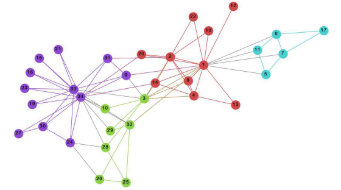
\includegraphics[width=\linewidth]{Figures/fig_karate_network.png}
  \caption{Karate network}
  \label{fig:karate_network}
\end{subfigure}%
\hspace{0.5cm}
\begin{subfigure}[t]{.5\textwidth}
  %\centering
  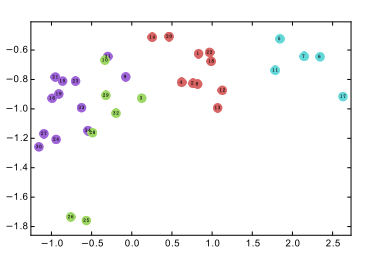
\includegraphics[width=\linewidth]{Figures/fig_karate_represtation.png}
  \caption{ The distributed representation of the karate network}
  \label{fig:karate_network_rep}
\end{subfigure}
 \caption{An example of a network embedding model. The image is extracted from~\protect\cite{DeepWalk}} 
  \label{fig:whole_karate_network_representation}
  %\cref{fig:whole_karate_network_representation}
\end{figure}




There are two main goals that network embedding models aim to achieve in order to represent the nodes in a low dimensional space~\cite{DBLP:journals/tkde/CuiWPZ19}:\\
\begin{enumerate}
  \item The original network can be reconstructed from the learned vector space, in other words, nodes that connected in the original network should be distance between them should be small.\\
  \item The learned embedding space should be applicable to original network inference task such as identifying important nodes.\\
\end{enumerate}

Network embedding models adopt different approaches, i.e., matrix factorization, random walk, deep neural networks, etc. in order to 
transfer the nodes into their low dimensional representation. In the following we give the most commonly used methods by the embedding models:\\
%different network embedding models adopt different approaches, i.e., matrix factorization, random walk, deep neural networks, etc. In this section we discuss the most commonly used approaches:  
\begin{itemize}
\item \textbf{Matrix Factorization.}\\
To represent a network topology matrices where each row and column corresponds to a node are commonly used~\cite{DBLP:journals/tkde/CuiWPZ19}. Each entry in this matrix indicates the relation between the corresponding nodes. Network embedding models aim to find the low dimensional representation of nodes of the given network. Matrix factorization methods are common ways to achieve this purpose. Given a matrix $M$, the matrix factorization can be defined as follows:\\ \begin{equation}\label{eq:matrix_factorization}
\min_{W, C} \Vert M - W^T C\Vert .
\end{equation}
where $W$ and $C$ are two matrices and have lower ranks than $M$. The matrix factorization operation given matrix $M$ aims to find $W$ and $C$ matrices.\\
%sepNE formula 1
\item \textbf{Random Walk.}\\
Random walks have been used in variety of applications such recommendation systems as a similarity measure~\cite{DeepWalk}. In the context of network embeddings, random walk models are being exploited to generate random paths over a given network. By doing so, neighbourhood information of vertices can be extracted from the network. Network embedding models which exploit random walk techniques mainly relies on the neighbourhood information of vertices in order to generate vector representation of vertices. This idea highly relates to a neural language model by regarding a vertex as a word and a random walk is a sentence then the node neighborhood can be identified by co-occurence rate as in Skip-Gram model~\cite{DBLP:journals/tkde/CuiWPZ19}.   \\
\item \textbf{Neural networks.}\\
Neural networks especially deep neural networks are also commonly exploited by the several network embedding models~\cite{}\todo{find embedding models as an example}. Section~\ref{} provides a general overview of neural networks. \\ 
\end{itemize}


In the following we give the example of the most prominent network embedding models applications:\\
\begin{itemize}
%cite each of them
\item \textbf{DeepWalk.}
DeepWalk network embedding model aims to learn distributed representation of vertices in a given network by considering the neighborhood relations of vertices. To this end, the model attempts to conduct two main tasks; first, the model generates random walks on a given network and secondly, the representation of each vertex which is generated by the random walks (from the first step) is updated based on a neural language model so called Skip-Gram (cf. Section). More precisely, DeepWalk relates the distribution of each vertex appearing in random walks to the distribution of words that appear in natural language~\cite{DBLP:journals/tkde/CuiWPZ19}. Motivated by this assumption, DeepWalk adapts a language model  to update the representation of each vertex generated by the random walks.
\begin{figure*}[h]
 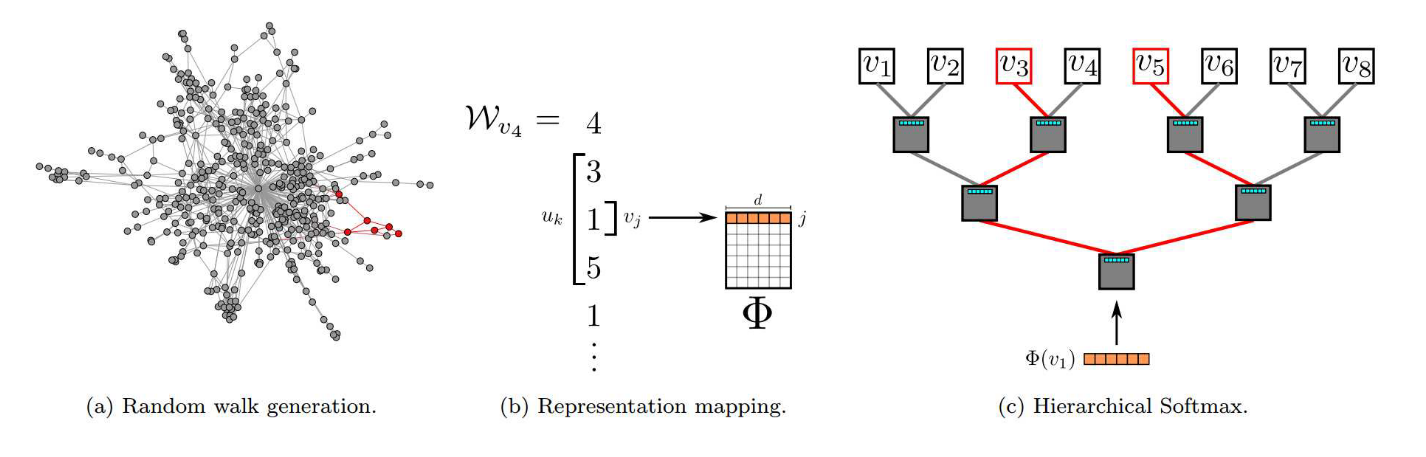
\includegraphics[width=\linewidth]{Figures/fig_deepwalk.png}
 \caption{An overview of DeepWalk architecture. The image is extracted from~\protect\cite{DeepWalk}.}
 \label{fig:deepWalk}
\end{figure*} \\
Figure~\ref{fig:deepWalk} depicts the overview of the DeepWalk model. Given a graph the random walk generator (Figure~\ref{fig:deepWalk}a) randomly samples a vertex $v$ as a root of the random walk $W$. Then the walk uniformly samples the neighbour of the last visited vertex iteratively until the maximum length of the walk $t$ is reached. The maximum length of the walks ($t$) is an input parameter. Likewise, the number of walks at each vertex $\gamma$ is also an input parameter.\\ 
Skip gram model iterates over all collection of vertices that appear within the given window size. In Section we have already \todo{Skip gram section, also check SkipGram vs Hsoftmax} introduced the Skip gram model, therefore, in this section we skip the technical details of it. As shown in Figure~\ref{fig:deepWalk}b each vertex $v$ is mapped to its  representation vector $\Phi(v)$. Finally, Hierarchical Softmax is used to learn the distributed representation of the vertices. \\
 
\item \textbf{LINE.}
Large-scale Information Network Embedding (LINE) learns latent representation of vertices of an arbitrary, i.e., undirected, directed, and/or weighted type of an information network. The model is capable of scaling to very large information networks. Moreover, LINE aims to optimize an objective function which preserves the local structure, i.e., \textit{first order proximity} and global structure, i.e., \textit{second order proximity} of a given network. 
\begin{figure*}[h]
\centering
 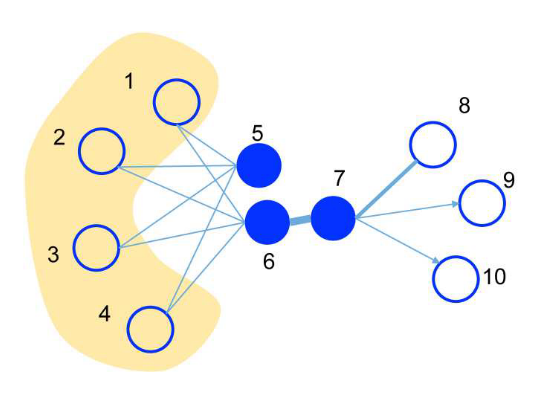
\includegraphics[height=5cm]{Figures/fig_LINE.png}
 \caption{An example of an information network. The image is extracted from~\cite{LINE}.}
 \label{fig:LINE}
\end{figure*} \\
Figure~\ref{fig:LINE} illustrates an example of a simple information network. The thickness of the edges between vertices determines the strongness of the connections. 
First order proximity defined as the observed local pairwise proximity between two nodes~\cite{DBLP:journals/tkde/CuiWPZ19}. For example, in Figure~\ref{fig:LINE} the observed edge between vertex 6 and 7 is stronger, i.e., thicker. According the first order proximity vertex 6 and 7 should be placed closely in the vector space. On the other hand, the first order proximity between the vertex 5 and 6 is zero as there is no edge between them.
To model the first order proximity between vertices $v_i$ and $v_j$ the following joint probability defined as:
\begin{equation} \label{eq:jointProb}
p_{1}(v_{i},v_{j})=\frac{1}{1+exp(-\vec{u}_{i}^{T}\cdot\vec{u}_{j})}
\end{equation}
where $\vec{u}_{i}$ ($\vec{u}_{j}$) is the vector representation of node $v_i$ ($v_j$), respectively. In addition, its empirical probability can be defined as $\hat{p_1}(v_i,v_j)=\frac{w_{ij}}{W}$, where $W=\sum_{(i,j) \in E}w_{ij}$, $E$ is the set of edges between nodes in the network, and $w_{ij}$ is the weight of the edge $(i,j)$.
In order to preserve the first-order proximity, the model aims to minimize the KL-divergence between the two distributions $p_{1}(v_{i},v_{j})$ and $\hat{p_1}(v_i,v_j)$. By omitting some constants, the final goal is to minimize the following objective function:
\begin{equation}
O_{1}=-\sum_{(i,j) \in E}w_{ij} \textrm{log}p_{1}(v_{i},v_{j})
\end{equation}
Note that the first order proximity only applicable for the undirected graphs.

Second order proximity is determined between the two vertices through the shared neighborhood structures of the vertices. In other words, two nodes considered to be similar if they share the same neighbors according to the notation of second order proximity. For example, the vertex 5 and 6 in Figure~\ref{fig:LINE} should be placed closely as they share similar neighbors. 
To model the second-order proximity, for each edge $(i,j)$, the conditional probability is defined as follows: 
\begin{equation}
p_{2}(v_{j}|v_{i})=\frac{exp(-\vec{u}_{j}^{T}\cdot\vec{u}_{i})}{\sum\limits_{k=1}^{|V|} exp(-\vec{u}_{k}^{T}\cdot\vec{u}_{i})}
%p_{1}(v_{j}|v_{i})=\frac{exp(-\vec{u}_{i}^{T}.\vec{u}_{j})}{\sum_{k=1}^{V}exp(-\vec{u}_{i}^{T}.\vec{u}_{j})}
\end{equation}
where $V$ is the set of nodes connected with $v_i$ in the network. The empirical probability of $p_{2}(v_{j}|v_{i})$ can be defined as $\hat{p_2}(v_{j}|v_{i})=\frac{w_{ij}}{d_i}$, where $d_i$ is the out-degree of $v_i$. In order to preserve the second-order proximity, the conditional distribution $p_{2}(v_{j}|v_{i})$ is made close to $\hat{p_2}(v_{j}|v_{i})$ based on the KL-divergence over the entire set of nodes in the network, such that the model minimizes the following objective function:
\begin{equation}
O_{2}=-\sum_{(i,j) \in E}w_{ij} \textrm{log} p_{2}(v_{j}|v_{i})
\end{equation}

In order to keep both first-order and second-order proximities for each node, two LINE models are trained. Firstly, a LINE model is trained by preserving the first-order proximity, and then another LINE model is trained by preserving the second-order proximity. Finally, concatenating the embeddings of both models yields an embedding for each node. \\

\item \textbf{Node2vec.}
Node2vec is based on the idea of learning the latent representation of the vertices in a given network by maximizing the likelihood of preserving network neighborhoods of vertices. Node2vec extends a prior work, i.e., DeepWalk, which is based on rigid notions of network neighborhoods. Unlike DeepWalk, node2vec designs a biased random walk procedure which explores diverse neighborhoods.  In other words, node2vec leverages \nth{2} order random walk approach to generate neighbourhoods for vertices\todo{nodes or vertices}. The key contribution of the model is biased random walk strategy which is capable of exploring diverse neighbours of vertices.\\  
Given a network $G = (V, E)$ where $V$ is all the vertices and $E$ is all the edges between the vertices in the network. Let $f : V \to \mathbb{R}^d$ be the function that maps the each vertex to its corresponding distributed $d$ dimensional vector representation. For each source node (the start node of a random walk) $u\in V$ , $N_s(u) \subset V$ is defined as network neighborhood of $u$ generated by biased random walk strategy $S$.\\
$S$ generates biased random walks in order to sample the neighborhood nodes that smoothly interpolate between breadth-first sampling (BFS) and depth-first sampling (DFS). 
Then, given a source node $u$ and the length $l$ of the walk, $c_i$ the $i_{th}$ node in the walk generated by the following distribution:


\begin{equation}
    P(c_i = x| c_{i-1}=v )= \begin{cases}
    \frac{\pi_{vx} }{Z}, & \text{if $(v,x)\in E$}.\\
    0, & \text{otherwise}.
  \end{cases}
\end{equation}

where $c_0 =u$, $\pi_{vx}$ is the transition probability between nodes $v$ and $x$, and $Z$ is the normalization constant. \\
Assuming a random walk traversed edge $(t, v)$ and now resides at node $v$. For the next step, the walk evaluates the transition probabilities on edges $(v,x)$ leading from $v$. Then the transition probability $\pi_{vx}=\alpha_{pq}(t,x)\cdot w_{vx}$ can be set as follows:
\begin{equation}
    \alpha_{pq}(t,x)= \begin{cases}
    \frac{1}{p}, & \text{if $d_{tx}$=0}.\\
    1, & \text{if $d_{tx}$=1}.\\
    \frac{1}{q}, & \text{if $d_{tx}$=2}.\\
  \end{cases}
\end{equation}
where $d_{tx}$ denotes the shortest path distance between nodes $t$ and $x$. The parameter $p$ controls the likelihood of immediately revisiting a node in the walk whereas $q$ allows the search to differentiate between inward and outward nodes.%“inward” and “outward” nodes.

Finally, the model tries to optimize the following objective function as follows:
\begin{equation}\label{eq:node2vec_objective}
\max_{f} \sum_{u \in V } \textrm{log} Pr(N_S(u)|f_{u})
\end{equation}

which maximizes the log-probability of observing a network neighborhood $N_S(u)$ for a node $u$ conditioned on its feature representation, given by $f$.\\
In order to optimize the above objective function two assumptions are made as:\\
\begin{itemize}
\item The likelihood of observing a neighborhood node is independent of observing any other neighborhood node as:
\begin{equation}
 Pr(N_S(u)|f(u))= \prod_{n_i \in N_S(u)}Pr(n_i|f(u))
\end{equation}
\item A source node and neighborhood node have a symmetric effect over each other in feature space and this assumption modeled as follows:

\begin{equation}
P_{r}(n_{i}|f(u))=\frac{exp(f(n_i)\cdot f(u))}{\sum\limits_{v \in V} exp(f(v)\cdot f(u))}
%p_{1}(v_{j}|v_{i})=\frac{exp(-\vec{u}_{i}^{T}.\vec{u}_{j})}{\sum_{k=1}^{V}exp(-\vec{u}_{i}^{T}.\vec{u}_{j})}
\end{equation}

\end{itemize}
Finally with the two above assumptions the Equation~\ref{eq:node2vec_objective} simplifies as follows:
\begin{equation}\label{eq:node2vec_objective_final}
\max_{f} \sum_{u \in V }[ -\textrm{log}Z_u + \sum_{n_i \in N_S (u) }f(n_i) \cdot f(u)]
\end{equation}
where $Z_u$ is a per\_node partition function which is $Z_u= \sum\limits_{v \in V} exp(f(v)\cdot f(u))$. The partition function $Z_u$ is expensive to calculate especially for the large networks, therefore, similar to Skip-gram model negative sampling method is adapted to approximate $Z_u$ function and stochastic gradient ascent is used to optimize the Equation~\ref{eq:node2vec_objective_final}.\\

%As it can be seen from the objective function~\ref{Equation 1} of the model is an extension of 
%Skip gram model. However, the neighbourhood sampling method $S$  is the key contribution of the model which generates biased random walks in order to sample the neighborhood nodes that smoothly interpolate between breadth-first sampling (BFS) and depth-first sampling (DFS). 

\item \textbf{SepNE.}
Given a network SepNE model learns the latent representation of vertices in subsets and in separeta processes. By doing so the model avoids the effort to embed the nodes that are irrelevant to the application at hand. Therefore, the model is capable of scaling to very large networks.\\
\begin{figure*}[h]
\centering
 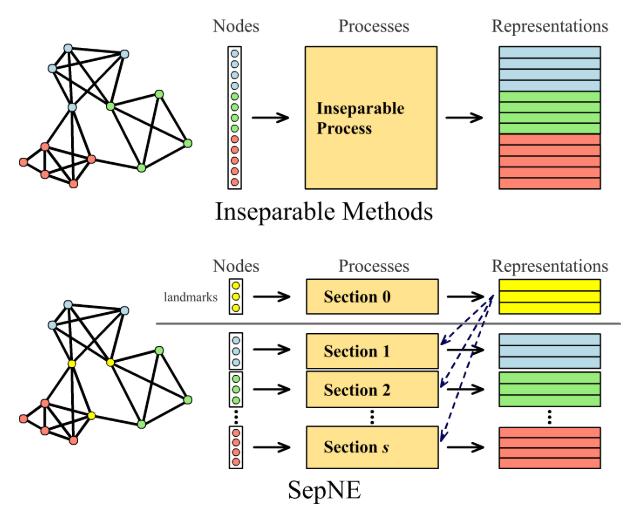
\includegraphics[height=5cm]{Figures/fig_SepNE.png}
 \caption{An example of Inseparable and separable network embedding processes. The image is extracted from~\protect\cite{SepNE}}
 \label{fig:SepNE}
\end{figure*} 
Figure~\cite{SepNE} depicts simple framework of SepNE and other models that do not separate the learning process. Traditional embedding models such as DeepWalk, LINE, node2Vec embed entire networks with inseparable processes. Unlike aforementioned models SepNE first, partitions the entire network into small subsets of nodes as shown in Figure~\ref{fig:SepNE}. A special set so called \textit{landmark set} which contains the highly interactive nodes in the network is constructed. The goal of the landmark set is to help for establishing references for different sets. First the landmark nodes are embedded, then the rest of the subsets are also embedded.\\
The model is formalized based on \textit{separated matrix factorization} (SMF). Let us first briefly explain matrix factorization (MF) . Given a matrix $M$ which is of size $(nxn)$, matrix factorization aims to reduce $M$ into its constituent parts $W$ and $C$ that both $W$ and $C$ satisfy given constraints in Equation~\ref{eq:matrix_factorization} for reconstructing $M$. On the other, separated matrix factorization takes a network $G=(V,E)$ its proximity matrix $M$ and the partition setup $f : V $ .. as inputs. The goal of SMF is then to drive representations $(W_1, ..., W_s)$ and $(C_1, ..., C_s)$ for the partitioned sets that optimally reconstruct $M$ as: \\
\[M=\begin{pmatrix}
M_{11} &\cdots &M_{1s} \\
\vdots & \vdots & \ddots & \vdots\\
M_{s1} &\cdots &M_{ss}
\end{pmatrix}\]
where $M_{ij}$ indicates the proximities between $V_i$ and $V_j$.  In the training phase, in order order to achieve independence between subsets, each embedding section of every set utilizes only the proximities related to itself, e.g, embeddin section $V_i$ can only utilize $M_{i1}, M_{i2}, M_{i3},..., M_{is}$. \\
The SMF model that preserves only local information i.e., proximities within every set and ignores the intractions between the sets modeled as follows:
\begin{equation}\label{eq:node2vec_objective_final}
\min_{W_i, C_i} \Vert M_{ii} - W_{i}^T C_i\Vert , i=1,..., s.
\end{equation}

Moreover, landmark set (denoted as $V_0$) is also used as an additional information to derive the representation of the subsets. Landmark nodes established to indicate the proximities between subsets. The embedding method of the model for landmarks can be formulated as :
\begin{equation}
\min_{\Phi, \Psi} \Vert M_{00} - \Phi^T \Psi \Vert ,
\end{equation}
Then the representation of rest of the subsets are derived accordingly as:
\begin{equation}\label{eq:sepne_landmark_subets}
\min_{W_i, C_i} \left\Vert 
\begin{pmatrix}
M_{00}  &M_{0i} \\
M_{i0} &M_{ii}
\end{pmatrix} - 
\begin{pmatrix}
\Phi^T \Psi & \Phi^T C_{i} \\
W_{i}^T \Psi & W_{i}^T C_{i}
\end{pmatrix} \right\Vert , i=1,..., s.
\end{equation}
Equation~\ref{eq:sepne_landmark_subets} can be decomposed into local and landmark loss as: 
%formula 4 and 5

\begin{equation}
\mathcal{L}_{i}^{lc}(W,C)=\frac{1}{2}\Vert M_{ii} - W_{i}^T C_i\Vert_{F}^2 
\end{equation}

\begin{equation}
\mathcal{L}_{i}^{lc}(W,C)=\frac{1}{2}\Vert M_{0i} - \Phi^T C\Vert_{F}^2 +\frac{1}{2}\Vert M_{i0} - W^T \Psi\Vert_{F}^2 
\end{equation}

Assume as a first stage  the landmarks $(W_0 = \Phi, C_0 = \Psi)$ are embedded. Let $W_i, C_i \in \mathbb{R}^{(d\times|V_i|)}$ represented as linear combination as:

\begin{align*}
& W_i= \Phi A_i \\
& C_i= \Psi B_i, i=1,..., s
\end{align*}
where $A_i, B_i \in \mathbb{R}^{(d\times|V_i|)}$
To further combine global information to derive the latent representation of the embeddings a global loss function defined as follows:
\begin{equation}
\mathcal{L}_{i}^{gb}(A,B)=\frac{1}{2}(\Vert M_{i\bar{i}} - A^T M_{0\bar{i}}\Vert_{F}^2 +\Vert M_{\bar{i}i} - M_{\bar{i}0}B\Vert_{F}^2)
\end{equation} 

Then the final loss function which is combined $\lambda-$scaled global loss of SMF becomes:

\begin{align*}
& W_0= \Phi C_0= \Psi . \\
& W_i= \Phi A_i, C_i= \Psi B_i \\
& A_i,B_i=\underset{A,B}{\mathrm{argmin}}\mathcal{L}_{i}(A,B),  i=1,..., s. 
\end{align*}


%\todo{Here we can add more emdedding models}

%\item \textbf{NetSMF.}

\end{itemize}
%DeepWalk, LINE, and node2vec


